% !TeX root = ../main.tex
% Add the above to each chapter to make compiling the PDF easier in some editors.


% \chapter{Explainability of Fake News Detection Models}\label{chapter:explainability_of_fnd_models}
% AI is getting more and more integrated into our lives, helping us with from the simplest tasks like playing music with voice command to more complex tasks like driving a car in open traffic.
% \section{Explainability of News Content Models}
% \label{sec:explainabilityOfNewsContentModels}
% \subsection{SHAP, DeepSHAP}

% \subsection{SHAP in Action}

% \subsection{Introducing Unseen Data}

% \subsection{Results}

% \section{Explainability of Social Context Models}

% \subsection{GNNExplainer}

% \subsection{GNNExplainer in Action}

% \subsection{Introducing Unseen Data}

% \subsection{Results}

\chapter{Mixed Approaches for Fake News Detection}\label{chapter:MixedApproachesForFND}

\section{Mixed Approaches}
\label{sec:mixedApproaches}
As discussed in Section~\ref{sec:fakeNewsDetection}, social media's interconnected nature leads to fast dissemination of
fake news. When a news piece is shared, it cascades through social media by means of friendship networks. These networks
can be exploited to gather information about how fake news spread. Moreover, a user's historical information can prove effective when trying to analyze whether a news piece is real or not. This assumption stems from the psychological facts we discussed in Section~\ref{sec:fakeNewsDetection}. To recap, if a user is sharing fake news most of the time, i.e., the user's tweets are marked as fake, then it is likely that the next news piece they share would be fake as well. Usually, fake news are shared most within echo chambers, which gives rise to quick spread of fake news.\\
There exist many different approaches for social context models, however, it is a long and challenging task to create a dataset for social context models as the amount of data to be collected can grow dramatically. Thus, we selected a dataset that provides us with the social context information as well as the news content. Being a graph dataset, \emph{User Preference-aware Fake Detection} (UPFD)~\parencite{UPFD_Dataset_Shu} builds a propagation tree for the news. But in order to build a model that takes graphs as input we can no longer rely on standard deep learning approaches as the graph data has a different structure than news content data. It holds node information as well as edge information between nodes, allowing to store rich relational data~\parencite{UPFD_Dataset_Shu}.\\
In this section, we lay out foundations for the dataset and GNNs we used. Then we talk about the social context models along with their dataset UPFD that we used in this thesis. We also give some insights from~\parencite{HierarchicalPropagationNetworksForFND_Shu} in which the authors of UPFD dataset analyze the data they later utilized to create the graph dataset UPFD.\\

\subsection{Overview of Graphs}
\label{subsec:mixedApproaches_OverviewOfGraphs}
In this section, we introduce definitions to cover graphs and different types of GNNs. But we do not discuss each model type in detail due to GNNs' extensive background. Thus, we do not provide a notation for this section but we give mathematical definitions when required.\\
Graphs are an example of \emph{non-euclidean} data, meaning that in contrast to \emph{euclidean} data, they can represent complex relations and entities more accurate than one or two dimensional representations. Non-euclidean data used in GDL can be grouped into grids, graphs, groups, geosedics, and gauges, which are also called the 5G's of \emph{Geometric Deep Learning} (GDL)~\parencite{GeometricDeepLearning_Bronstein}. We are interested in one G only, graphs.
\begin{definition}[\emph{Geometric Deep Learning (GDL)}]
    A class of deep learning that aims to build models that can learn to predict on the non-euclidean domain.
\end{definition}
GDL is an extensive field covering various techniques that can be appied to non-euclidean domain. Due to its complex nature, we do not provide a rigorous background on GDL. For a detailed background on GDL, we refer the reader to an extensive study on GDL~\parencite{GeometricDeepLearning_Bronstein}. We only discuss parts related to GNNs that we utilized. First we define a graph.
\begin{definition}[\emph{Graph}]
    A graph is a non-euclidean type of data that represents the relations between entities.
\end{definition}
From the perspective of individual node connections, graphs can be categorized into two classes, \emph{directed} and \emph{undirected} graphs. Directed graphs have direction information in their edges, i.e., the information flows strictly from one node to another. On the other hand, undirected graphs do not have this limitation, the information flow is bidirectional. Since we are only interested in undirected graphs like our dataset, we give preliminaries for an undirected graph.\\
Following common notation on graphs, we define an undirected graph as $\mathcal{G} = (\mathcal{V}, \mathcal{E})$ with $\mathcal{V}$ as the set of nodes and $\mathcal{E}$ as the set of edges in a graph $\mathcal{G}$. We say that an edge $(v_i, v_j)$ exists between two nodes $v_i$ and $v_j$. Moreover, from the perspective of a graph's connectedness, there exist two types of graphs, \emph{cyclic} or \emph{acycylic}. Simply put, cyclic graphs have cycles in them, i.e., the graphs allows for at least one node $v_i$ to have a series of different edges that creates a cycle back to the node $v_i$. In contrast, acyclic graphs do not contain cycles. A concrete example for undirected acyclic graphs are trees. Also the structure of our dataset, trees have strictly one edge between two nodes.\\
When we look at graphs from node and edge type, we classify graphs as \emph{homogeneous} and \emph{heterogeneous} graphs. Homogeneous graphs have nodes and edges of the same type, whereas heterogeneous graphs have different types of nodes and edges. One example for homogeneous graphs are social networks in which the nodes are users and the edges represent the friendship between two users. If we modify this social network into a more detailed version in which we choose to represent another relationship between users, such as colleagueship, then we would have a heterogeneous graph, because there would be two types of edges in the graph.\\
Finally, if we consider graphs from a temporal aspect, we observe two kinds of graphs, \emph{static} and \emph{dynamic}. Static graphs stay the same over time, their topology or features do not change. In contrast, dynamic graphs' features and topology vary  over time, thus making time an important factor when working with dynamic graphs.

\subsection{Graph Neural Networks}
\label{subsec:mixedApproaches_GraphNeuralNetworks}
GNNs are neural networks that can take graphs as an input and produce predictions at three different levels:
\emph{node-level}, \emph{edge-level}, and \emph{graph-level}. Node-level tasks include node classification, node
regression, node clustering. Node classification aims to categorize nodes into classes. Node regression deals with
predicting continuous value for each node. Lastly, node clustering aims to group nodes into several clusters. Edge-level tasks consist of edge classification and link prediction. Edge classification tries to categorize an edge. Link prediction aims to find whether there is an edge between two nodes. Graph-level predictions are graph classification, graph regression, and graph matching. In all these settings, the model needs to learn representations of graph~\parencite{GNNsAReview_Zhou}.\\
In our experiments, we used two different models one of which uses a convolutional layer called GraphSAGE~\parencite{GraphSAGE_Hamilton} and the other uses a convolutional attention layer called \emph{Graph Attention} (GAT)~\parencite{GraphAttentionNetworks_Velickovic}. Here we give background for both but we do not dive into details. We first give information about general framework.\\
\cite{GNNsAReview_Zhou} defines three modules that are involved in a generic GNN model: \emph{propagation module}, \emph{sampling module}, \emph{pooling module}. Propagation module deals with information propagation between nodes so that the aggregated information can represent features and topology of the graph. Propagation modules usually employ a \emph{convolution operator} or \emph{recurrent operator} to aggregate information from neighbors of nodes. These aggregated values are then used to update the representation of the nodes, edges, and graph. Additionally these modules employ a skip connection that helps collect previous representations of nodes to alleviate the over-smoothing problem. Sampling module is used when the input graph is large to handle propagation. It is used before propagation module. Lastly, pooling modules are employed when we need to extract information to represent high-level graphs.\\
We will mostly deal with propagation module and the operations within. We do not dive into mathematical background of convolutions in detail but we introduce mathematical formulations in order to illustrate the operations our models are using. Also, we do not discuss recurrent operations on graphs as their background is extensive and out of scope of this thesis. We refer the reader to~\cite{GNNsAReview_Zhou} for an extensive mathematical baackground on convolutions and other operations on spectral domain. However, we will summarize the behavior of convolutions on graphs in order to give the sufficient knwoledge for the models we used.\\
\textbf{Convolutions on graphs.} The idea of convolution operators is to generalize convolutions from another domain to spectral domain. In general there are two types of convolutional operations.\\
The first, \emph{spectral approaches}, are based on graph signal processing and defines its convolutional operators in the spectral domain~\parencite{TheEmergingFieldOfSignalProcessingOnGraphs_Shuman}. Spectral methods initially transform a graph signal $x$ to the spectral domain by the graph Fourier transform $\mathcal{F}$, then the convolution operation is applied. The output from convolution is transformed back with the inverse Fourier transform $\mathcal{F}^{-1}$. Now we summarize the mathematics behind this approach in order to convey our models' characteristics. Graph Fourier and inverse graph Fourier transform are defined as,
\begin{center}
    $\mathcal{F}(x) = U^T x$
\end{center}
\begin{center}
    $\mathcal{F}^{-1}(x) = Ux$
\end{center}
where $U$ is the eigenvalue matrix of normalized graph Laplacian $L = I_N - D^{\frac{-1}{2}} A D^{\frac{-1}{2}}$ with $I_N$ the identity matrix of dimension $N$, $D$ as the degree matrix and $A$ as the adjacency matrix of the graph. $L$ is a real symmetric positive semi-definite matrix which helps us with factorization $L = U \Lambda U^T$ where $\Lambda$ denotes the diagonal eigenvalue matrix~\parencite{GNNsAReview_Zhou}. Now that we can convert our graph signal $x$ to spectral domain and back, following~\cite{AWaveletTourOfSignalProcessing_Mallat} and~\cite{GNNsAReview_Zhou}, we can define the convolution operation on $x$.
\begin{center}
    $g \star x = \mathcal{F}^{-1}(\mathcal{F}(g) \bigodot \mathcal{F}(x))$ \\ $= U(U^T g \bigodot U^T x)$
\end{center}
where $\bigodot$ stands for element-wise multiplication and $U^Tg$ is the convolution filter in the spectral domain. This can be further simplified into the basis function of spectral methods:
\begin{center}
    $g_w \star x = U g_w U^T x$
\end{center}
where $g_w$ is a diagonal learnable matrix. Essentially, all spectral methods use a convolutional filter $g_w$ but their choice of design creates a variety of approaches that are built upon each other. We only discuss the ones necessary for our models. The main idea of modern convolutional operators come from approximating $g_w$ with $k$-th order Chebsyshev polynomials. GCN adopts $k=1$ to avoid overfitting. Moreover, it introduces a renormalization trick to solve the exploding/vanishing gradient problem~\parencite{GCN_Kipf}. Further works like AGCN~\parencite{AGCN_Li} have employed a similar approach. Additionally, GCN is employed to an extent in spatial approaches.\\
The second, \emph{spatial approaches} focus on the graph structure. They define convolutions directly on graph topology. Spatial approaches can be grouped into \emph{basic}, \emph{attention-based}, and \emph{framework}. Basic spatial approaches define convolution operations on the neighborhoods of different sizes. Neighborhoods are defined based on nodes as follows $\mathcal{N}_v$ for a node $v$. There exist several basic spatial approaches such as the diffusion CNN (DCNN)~\parencite{DCNN_Atwood} which describes the neighborhhood for nodes using transition matrices, the learnable GCN (LGCN)~\parencite{LGCN_Gao} which utilizes CNNs as aggregators by applying max pooling on neighborhhood matrices.\\
Another example, GraphSAGE uses an inductive learning approach to sample then aggregate features from a node's local neighborhhood. GraphSAGE uniformly samples a fixed-size collection of neighbors then aggregates this collection to produce embeddings for the graph~\parencite{GraphSAGE_Hamilton}. More precisely, let us assume that we have learned the parameters of $K$ aggregator functions denoted as $\textsc{AGG}_k$, and a set of weight matrices $W^k$ where $\forall k \in \{1, \dots K\}$. $k$ can be referred to as layer or search depth. Then for each $k$ we go through all nodes $v \in \mathcal{V}$ and apply an aggregation then an update. Concretely, at each $k$ and at each $v$, let $h_v^{k-1}$ denote the hidden state of a node $v$ at layer $k-1$. Following the same notation, we refer to the hidden state of a node's neighborhood $\mathcal{N}_v$ at layer $k$ as $h_{\mathcal{N}_v}^k$. GraphSAGE formalizes its aggregation and update operation at layer $k$ as:
\begin{center}
    $h_{\mathcal{N}_v}^{k} = \textsc{AGG}_{k}(\{h_u^{k-1}, \forall u \in \mathcal{N}_v\})$
\end{center}
\begin{center}
    $h_v^k = \sigma(W^k [h_v^{k-1} || h_{\mathcal{N}_v}^k])$
\end{center}
where $||$ denotes concatenation of two vectors, $[h_v^{k-1} || h_{\mathcal{N}_v}^k]$ concatenated vector and $\sigma$
a non-linear activation function. GraphSAGE employs three different aggregators: \emph{mean aggregator}, \emph{LSTM aggregator}, and \emph{pooling aggregator}. Mean aggregator collects sampled neighborhood information and takes the element-wise mean of the vector set $\{h_u^{k-1}, \forall u \in \mathcal{N}_v\}$. The inductive version also includes previous layer representation of node $v$, $h_v^{k-1}$. LSTM aggregator uses an LSTM to collect neighborhood information. LSTMs are more expressive than mean aggregators. However, since LSTMs are not permutation invariant, i.e., they process
their inputs sequentially, they need a modification to work with unordered sets. Finally, pooling aggregator first independently feeds each neighbor's vector to a FCN, then apply a pooling operation on the output.\\
The third, \emph{attention-based approaches}, utilizes the same attention logic introduced in~\ref{subsec:newsContentModels_TransformerArch} by following~\cite{NeuralMachineTranslationByJointlyLearning_Bahdanau}. A recent work Graph Attention Networks (GAT)~\parencite{GraphAttentionNetworks_Velickovic} proposes to integrate attention into the propagation step by computing the hidden state for node $v$ at layer $k$ as follows:
\begin{center}
    $h_v^{k} = \sigma(\sum\limits_{u \in \mathcal{N}_v} a_{vu} W h_u^k)$ \\
\end{center}
\begin{center}
    $\alpha_{vu} = \dfrac{exp(LeakyReLU(a^T[Wh_v || Wh_u]))}{\sum\limits_{k \in \mathcal{N}_v}exp(LeakyReLU(a^T[W h_v || W h_k]))}$
\end{center}
with $W$ as the weight matrix, $a$ as the weight vector of feed forward network and the non-linear activation function LeakyReLU is defined as:
\begin{center}
    \[LeakyReLU(\gamma, x) =
        \begin{cases}
            x,         & if x \geq 0 \\
            \gamma  x, & otherwise   \\
        \end{cases}
    \]
\end{center}
The authors in~\cite{GraphAttentionNetworks_Velickovic} also utilize Multi-Head Attention in order to stabilize the
learning process of attention(also called self-attention or intra-attention)~\parencite{AttentionIsAllYouNeed_Vaswani}. Concretely, same as GraphSAGE defined $K$ aggregators, GAT defines $T$ independent attention heads to compute hidden states and then features of these hidden states are either concatenated,
\begin{center}
    $h_v^k = ||_{t=1}^T \sigma(\sum\limits \alpha_{vu}^t W_t h_u^k)$
\end{center}
or averaged,
\begin{center}
    $h_v^k = \sigma(\frac{1}{T} \sum\limits_{t=1}^T \sum\limits_{u \in \mathcal{N}_v} \alpha_{vu}^t W_t h_u^k)$
\end{center}
to obtain the output where $\alpha_{vu}^t$ represents the normalized attention values of the attention head $t$.\\
The last convolutional spatial approaches cover general frameworks that aims to integrate multiple different models into one framework. A mixture model MoNet was proposed by~\cite{GeometricDeepLearningOnGraphsAndManifolds_Monti} which is a spatial framework for unifying models such as GCN~\cite{GCN_Kipf}, ~\cite{GeodesicCNNsOnRiemannManifolds_Masci}, DCNN~\cite{DCNN_Atwood} and many more in non-euclidean domain.\\
One more thing we need to investigate is graph sampling in order to cover everything that was utilized in this thesis. GNN models suffer from an issue called \emph{neighbor explosion} which stems from having massive sizes of supporting neighbors from all previous layers as the number of layers increases~\cite{GNNsAReview_Zhou}. Likewise, as graph size increases, we will encounter the same problem. Sampling is used to solve this issue and it can be done on three levels: \emph{node sampling}, \emph{layer sampling}, and \emph{subgraph sampling}. Node sampling creates a subset using the neighborhood set $\mathcal{N}_v$ of the node's $v$. As discussed previously, GraphSAGE~\parencite{GraphSAGE_Hamilton} employs node sampling. Layer sampling takes a different approach and it selects a subset of nodes for aggregation. Lastly, subgraph sampling deals with the graph as a whole. One approach is to use clustering algorithms to obtain these subgraphs~\parencite{ClusterGCN_Chiang}. Another is to sample nodes and edges from graph to create a subgraph~\parencite{GraphSAINT_Zeng}.\\

\subsection{Dataset and Models}
\label{subsec:mixedApproaches_DatasetAndModel}
Our choice of dataset, UPFD~\parencite{UPFD_Dataset_Shu} utilizes the dataset FakeNewsNet~\parencite{FakeNewsNet_Shu}. From FakeNewsNet, the authors of UPFD build a graph dataset by collecting user preference information from historical posts and social context data with Twitter Developer API~\parencite{TwitterAPI_Twitter}. They further employ textual embedding techniques to encode historical posts and news content. We shall discuss how these operations are conducted in detail. UPFD has two three preparation levels which the authors coined as \emph{endogeneous preference encoding}, \emph{exogeneous context extraction}, and \emph{information fusion}. The framework is shown in Fig~\ref{fig:UPFD_Framework}\\
\begin{figure}
    \centering
    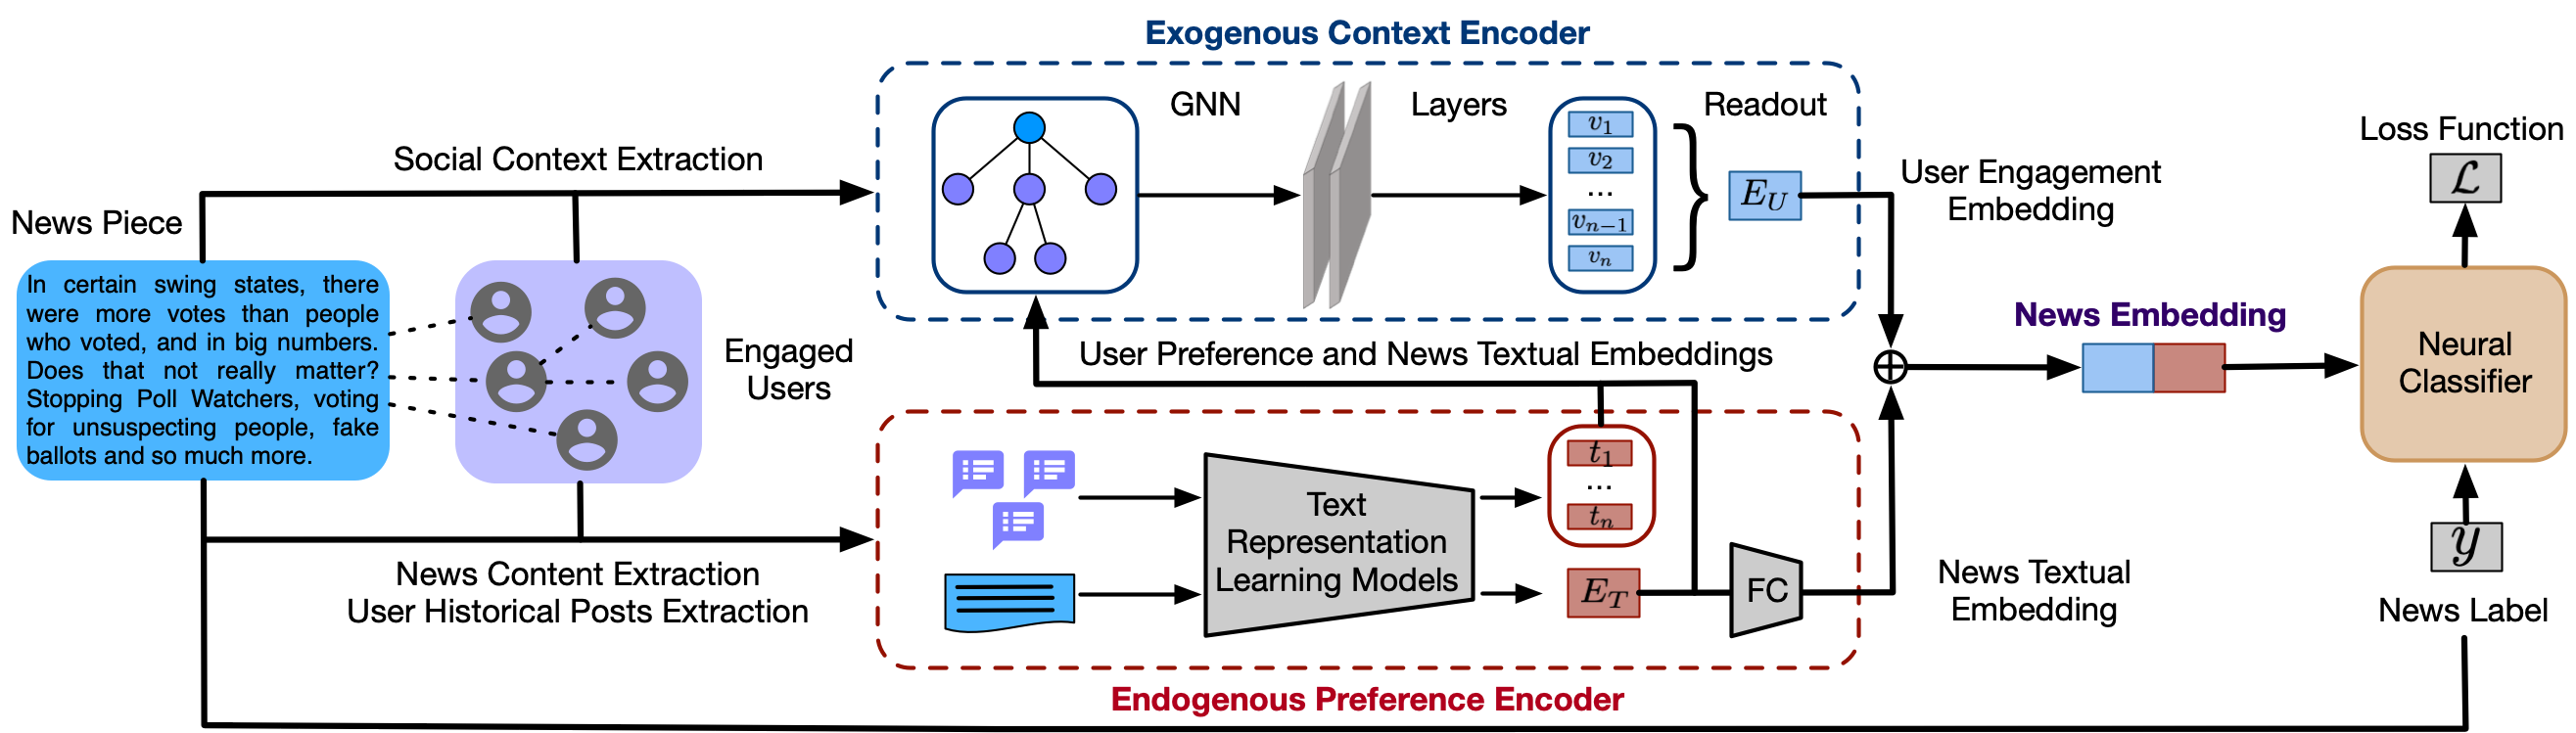
\includegraphics[scale=0.33]{UPFDFramework.png}
    \caption[UPFD Framework]{The framework of UPFD. Image obtained from~\parencite{UPFD_Dataset_Shu}}
    \label{fig:UPFD_Framework}
\end{figure}
\textbf{Endogeneous preference encoding} deals with user historical posts and news content using the news content and social engagement data in FakeNewsNet. With social engagement data, the authors collect 200 historical tweets of each user who have retweeted the news in FakeNewsNet. Summing up to almost 20 million tweets, these collection procedure of historical tweets for each FakeNewsNet news instance is as follows~\parencite{UPFD_Dataset_Shu}:
\begin{itemize}
    \item Collect user ids who have retweeted.
    \item For each user, collect 200 most recent tweets.
    \item For inaccessible (suspended or deleted) users, use randomly sampled tweets from accessible users who engage the same news piece. This step also increases the effectiveness of the exogeneous encoder.
    \item  Finally, remove special characters such as "@" and URLs before applying textual techniques.
\end{itemize}
Now that we have news content and user historical information, we encode these texts using text representation learning techniques. Still following~\cite{UPFD_Dataset_Shu}, the authors define two different settings for creating endogeneous preference encoding. The first setting, \emph{spacy}, deals with obtaining the representation for user historical data and news content with spaCy~\parencite{SpaCy_Honnibal} pretrained 300-dimensinal vectors for 680K words. For each user historical post (and similary for each news piece), if a word appears in the text, we include the vector for that word for final calculation in which all included vectors are averaged. As a result, we obtain a 300-dimensinal vector for each user historical information and news piece. The second setting, \emph{bert}, uses BERT-Large model to encode news and historical user data. Using bert-as-a-service~\parencite{BertAsAService_Xiao}, the authors encode the news content with maximum input sequence length as 768. To encode historical information, the authors opt for a different setting since 200 tweets cannot be processed as a single document due to BERT's maximum input sequence length limitation of 768. It is important to note that the paper of UPFD~\parencite{UPFD_Dataset_Shu} states the maximum input sequence length as 512, however in the dataset itself, the maximum sequence length is 768~\parencite{UPFD_PyGTeam}. Keeping in mind that tweets are usually short texts compared to news pieces, the authors use maximum input sequence length of 16 for each historical tweet, then average all 200 tweets to obtain the final representation for user historical data. This representation is of the same dimension as the root news node. Note that these text representation vectors are node features of a hierarchical tree structured graph whose root node represents the news content and the children of root represent the users who have retweeted.\\
\textbf{Exogeneous context extraction} uses retweet information to build the previously mentioned hierarchical tree. The authors adopt a similar procedure used in~\cite{GraphNeuralNetworksWithContinualLearningFakeNewsDetection_Han,GeometricDeepLearningOnGraphsAndManifolds_Monti,HierarchicalPropagationNetworksForFND_Shu}. In detail, authors define a news piece as $v_1$ and the set of users who retweeted $v_1$ as $\{v_2, \dots , v_n\}$ ordered by time. The rules are defined for this process to cover edge cases as well:
\begin{itemize}
    \item Estimate that a news piece propagates to user $v_i$ from user $v_j$ with the latest timestamp, if any user from the set $\{v_j | j\in \{2, \dots, n\}\setminus \{i\}\}$ retweeted the news piece before the user $v_i$. This conservative assumption is based on the fact that latest tweets are presented to the user first in the Twitter app~\parencite{UPFD_Dataset_Shu}.
    \item If user $v_i$ does not follow any users in the set $\{v_1, \dots, v_n \} \setminus {i}$, i.e., all retweeters and news source except the user itself, the authors approximate the spreader of that news piece to user $v_i$ as the user with most followers in the set. This approximation is based on the phenomena that the tweets from accounts with more followers have a higher probability of being retweeted or viewed.
\end{itemize}
After this procudure, we have our hierarchical tree for each news obtained from FakeNewsNet which employs two sources: Politifact and Gossipcop. Thus, we evaluate these datasets separately within UPFD. The distribution of the instances with respect to train/val/test split and label is provided in Fig.~\ref{fig:UPFD_Dataset_Visualization}.\\
\begin{figure}
    \subfloat[Gossipcop]{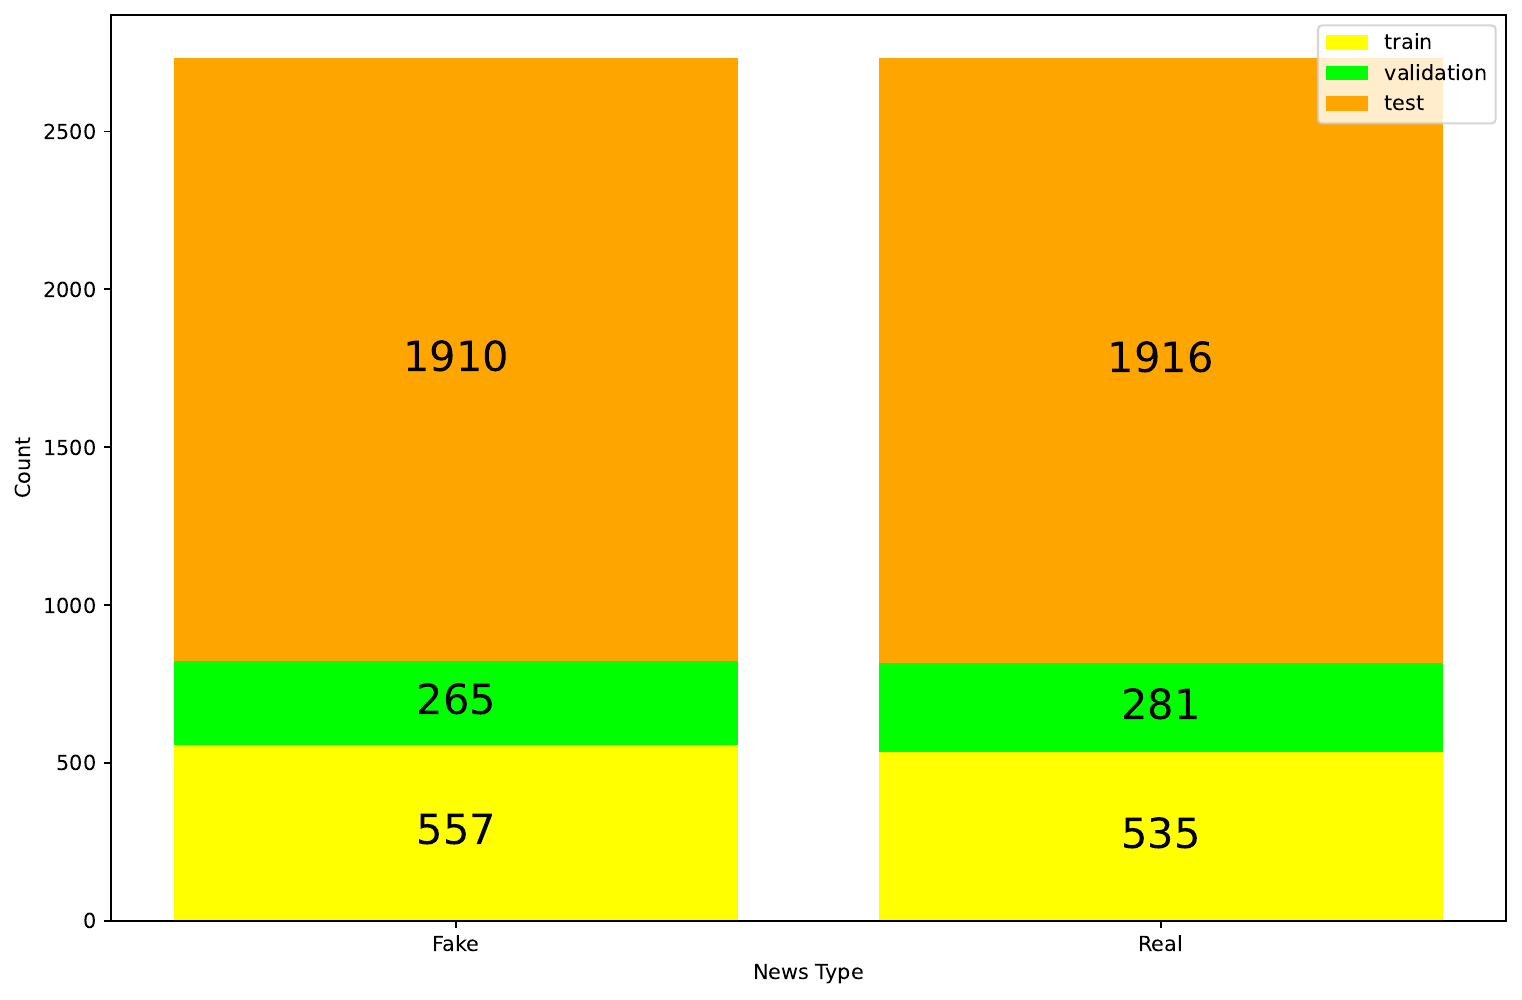
\includegraphics[width=0.45\textwidth]{GOS_DatasetDistrByLabelAndSplit.png}}
    \hfill
    \subfloat[Politifact]{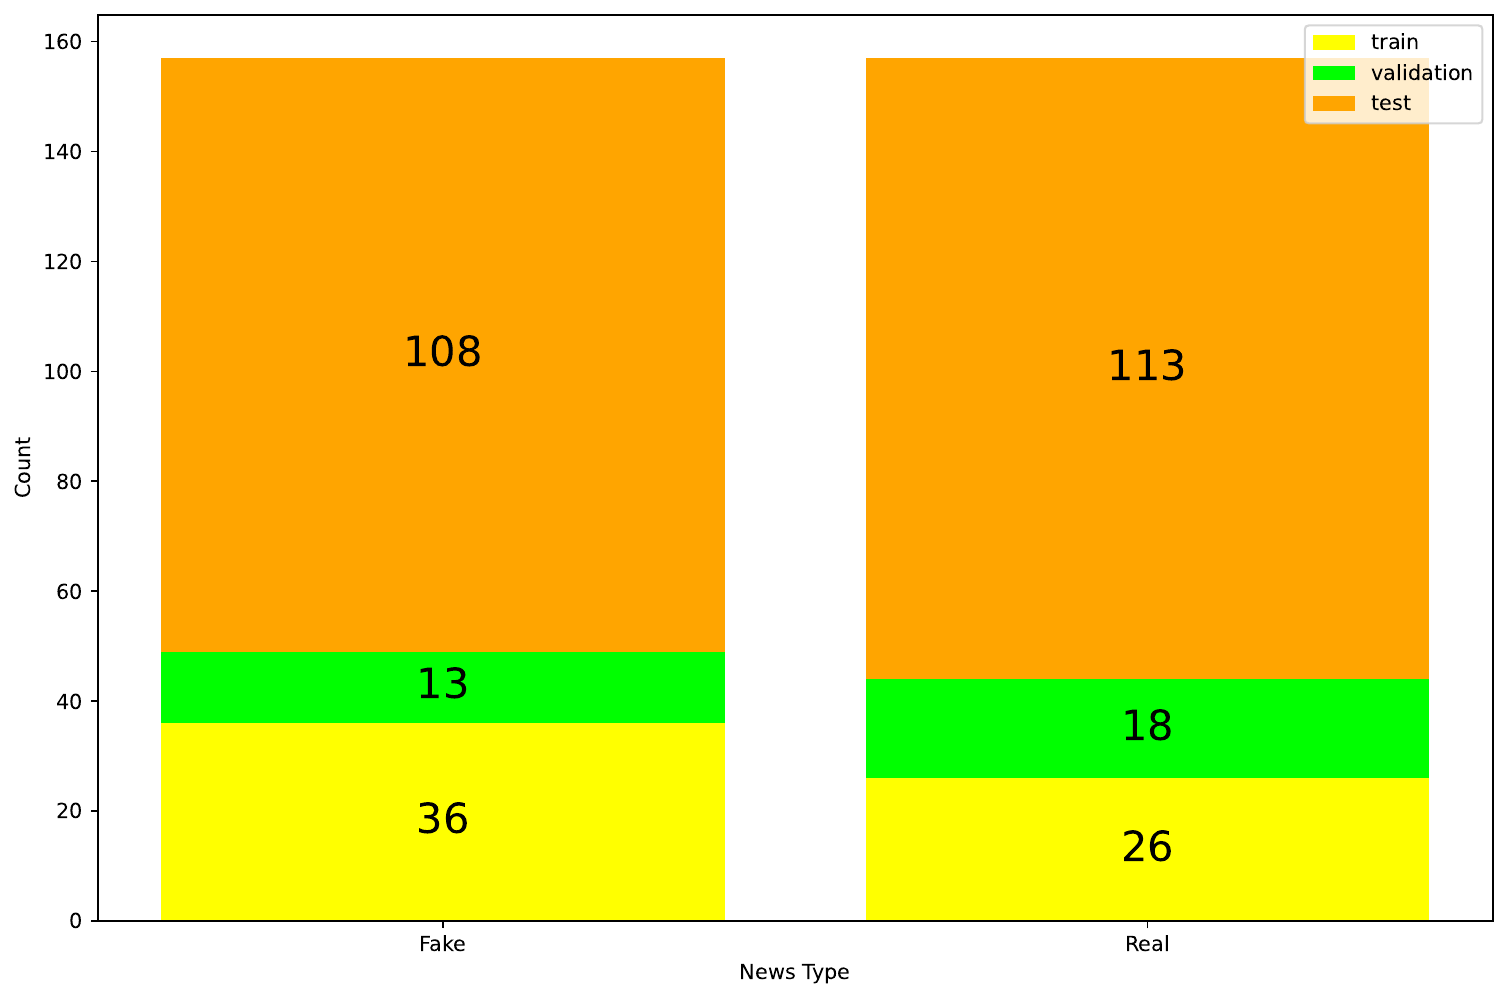
\includegraphics[width=0.45\textwidth]{POL_DatasetDistrByLabelAndSplit.png}}
    \caption[UPFD dataset distribution by label and split]{UPFD dataset distribution by label and split (train: 20\%, val: 10\%, test: 70\%)}
    \label{fig:UPFD_Dataset_Visualization}
\end{figure}
\textbf{Information fusion} is achieved via GNNs. As discussed in~\ref{subsec:mixedApproaches_GraphNeuralNetworks}, GNNs can encode graphs by maintaining the node features and structural information. From this point on, we need to utilize the models we introduced with a classification setting. Classification is done for each graph which represents the diffusion tree of the news piece~\parencite{UPFD_Dataset_Shu}. We adopted two models from this work's ablation study, the first one is based on GraphSAGE~\parencite{GraphSAGE_Hamilton}, and classification is handled with an FCN. We use BERT as the encoder since the best performance is obtained via that according to the experiments in~\cite{UPFD_Dataset_Shu} and the experiments we conducted. We call this model UPFD model as authors did in~\cite{UPFD_Dataset_Shu}. It is illustrated on Fig~\ref{fig:UPFDClassifierArchitecture}.
\begin{figure}
    \centering
    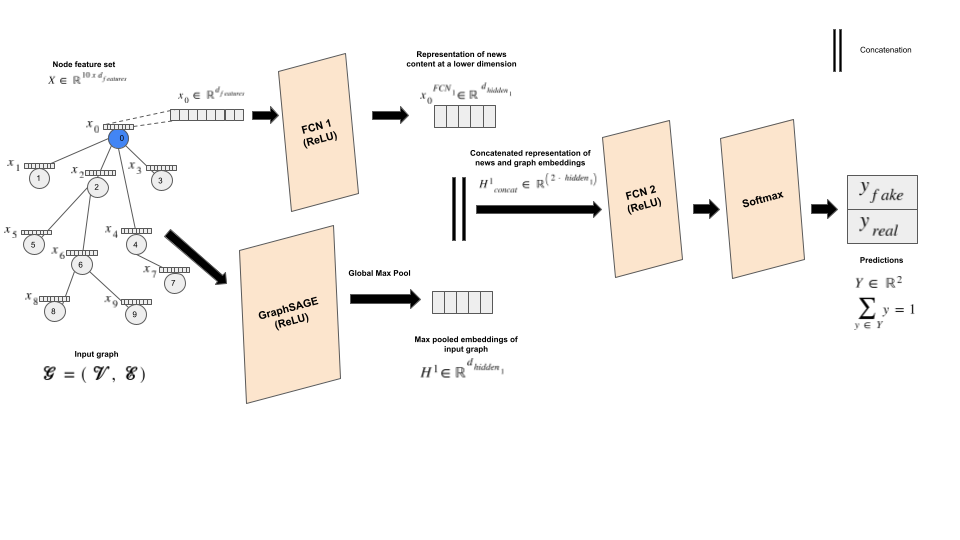
\includegraphics[scale=0.43]{UPFDClassifierArchitecture}
    \caption[UPFD classifier model pipeline]{UPFD classifer model pipeline. We used an example input graph with 10 nodes. $d_{hidden_1} = 128$ stands for hidden layer dimension of FCN 1, accordingly, $d_{hidden_2} = 128$ for the hidden dimension of FCN 2, and $d_{feature} = 768$ for feature dimension.}
    \label{fig:UPFDClassifierArchitecture}
\end{figure}
After obtaining the graph encodings, the authors suggest to concatenate a representation of news content with graph embeddings. More precisely, the feature vector of root node is fed to an FCN to obtain a lower-dimensional representation which is then concatenated with graph embeddings. The concatenated vector is then fed to another FCN, and lastly the softmax layer for classification. With the setting illustrated in Fig~\ref{fig:UPFDClassifierArchitecture}, the optimizer as Adam with default $\beta_1$ and $\beta_2$, and hyperparameters provided in Table~\ref{tab:UPFDClassifier_Hyperparameters},
\begin{table}
    \centering
    \begin{tabular}{|l|l|}
        \hline
        Activation function & ReLU~\parencite{ReLU_Nair} \\
        \hline
        Batch size          & 128                        \\
        \hline
        Epochs              & 35                         \\
        \hline
        Learning rate       & 0.01                       \\
        \hline
        Hidden layer 1 size & 128                        \\
        \hline
        Hidden layer 2 size & 128                        \\
        \hline
        Weight decay        & 0.01                       \\
        \hline
    \end{tabular}
    \caption[Hyperparameters of UPFD classifier.]{Hyperparameters of UPFD classifier.}
    \label{tab:UPFDClassifier_Hyperparameters}
\end{table}
we obtain 95.49\% and 83.16\% accuracy from Gossipcop and Politifact averaged by 10 runs, respectively. All other statistics are provided in Table~\ref{tab:UPFDClassifier_Results}.
\begin{table}
    \centering
    \begin{tabular}{c | c | c | c | c}
        \textbf{Dataset} & \textbf{Accuracy} & \textbf{Precision} & \textbf{Recall} & \textbf{F1 score} \\
        \hline
        Gossipcop        & 95.49\%           & 94.95\%            & 96.17\%         & 95.50\%           \\
        \hline
        Politifact       & 83.16\%           & 84.05\%            & 82.19\%         & 83.25\%           \\
    \end{tabular}
    \caption[UPFD classifier performance metrics averaged over 10 runs.]{UPFD classifier performance metrics averaged over 10 runs.}
    \label{tab:UPFDClassifier_Results}
\end{table}
Before we investigate what our classifier takes into account when classifying this news instance as fake news, we will summarize some of the features of our dataset which are proven to have significant effect by statistical tests in~\cite{HierarchicalPropagationNetworksForFND_Shu}.\\
~\cite{HierarchicalPropagationNetworksForFND_Shu} proposes to create two levels of propagation networks, \emph{macro-level} and \emph{micro-level}, using FakeNewsNet~\parencite{FakeNewsNet_Shu}. For each level, the authors define and statistically test the significance of a set of features. We want to see if some of those features are adopted by our classififer. Briefly, macro-level networks are constructed to track the cascade of a news piece via retweets, whereas micro-level propagation networks are built using the replies to retweets. UPFD is the macro-level propagation network, thus our focus is on the features of macro-level propagation network.\\
The features are macro-level propagation networks are categorized into two: \emph{structural} and \emph{temporal}. Structural features capture the patterns in global dissemination of a news piece~\parencite{HierarchicalPropagationNetworksForFND_Shu}. These features include:
\begin{itemize}
    \item ($SF_1$) \emph{Tree Depth}: Indicates how far the news piece has spread through the propagation network~\parencite{HierarchicalPropagationNetworksForFND_Shu}.
    \item ($SF_2$) \emph{Number of nodes in macro-network}: Indicates how many users have shared the news piece~\parencite{HierarchicalPropagationNetworksForFND_Shu}.
    \item ($SF_3$) \emph{Maximum outdegree}: Helps reveal the tweet/retweet with the most influence in the propagation network~\parencite{HierarchicalPropagationNetworksForFND_Shu}.
    \item ($SF_4$) \emph{Number of cascades}: The number of tweets that post the original news article~\parencite{HierarchicalPropagationNetworksForFND_Shu}.
    \item ($SF_5$) \emph{Depth of node with maximum outdegree}: Indicates steps of propagation required for a news piece to be retweeted by an influential user (node) whose post is retweeted by more users than any other users' retweet~\parencite{HierarchicalPropagationNetworksForFND_Shu}.
    \item ($SF_6$) \emph{Number of cascades with retweets}: Indicates the number of tweets shared the original news article and retweeted at least once~\parencite{HierarchicalPropagationNetworksForFND_Shu}.
    \item ($SF_7$) \emph{Fraction of cascades with retweets}: Corresponds to $SF_6 / SF_4$~\parencite{HierarchicalPropagationNetworksForFND_Shu}.
    \item ($SF_8$) \emph{Number of bot users retweeting}: Captures the number of bot users that retweeted that news piece~\parencite{HierarchicalPropagationNetworksForFND_Shu}.
    \item ($SF_9$) \emph{Fraction of bot users retweeting}: Corresponds to $SF_8 / SF_2$~\parencite{HierarchicalPropagationNetworksForFND_Shu}.
\end{itemize}
First of all, the feature set is not restricted to these features, one can derive more features for this dataset. We
will investigate some of these features in order to understand whether we can capture similar feaures in our explanations.
We do not have access to the information of bot users in our dataset, thus we drop the analysis of features $SF_8$ and $SF_9$. Additionally, we did not analyze temporal features as obtaining them from the explanation proved to be a long process. We now discuss which features' average values are found to be significant by statistical tests in~\parencite{HierarchicalPropagationNetworksForFND_Shu}. First structural feature $SF_1$ is found to be consistently different for
real and fake news instances in both datasets Gossipcop and Politifact under statistical t-test~\parencite{HierarchicalPropagationNetworksForFND_Shu}. Concretely, this finding indicates that tree depth of fake news are larger
than that of real news. Next, another simple feature $SF_2$ is also shown to be consistently different, particularly fake news instances have less nodes than real news instances. Although helpful, without additional information this feature is
too broad. Thus, we look at the next structural feature $SF_3$. It is found in~\parencite{HierarchicalPropagationNetworksForFND_Shu} that this feature consistently different for fake and real news in Gossipcop under t-test. More precisely, it is found that the maximum outdegree is bigger in fake news instances of Gossipcop. Considering this observation, we now proceed to more complex features.\\
When we look at features that analyze more subtle properties of the dataset such as $SF_5$ and $SF_7$, it is reported that these features are also consistently different for fake and real news instances from both datasets Politifact and Gossipcop~\parencite{HierarchicalPropagationNetworksForFND_Shu}.According to the study, $SF_5$ is discovered to be bigger in fake news, i.e., the finding suggests fake news reach the users from another user who retweeted the original fake news instance. The other feature $SF_7$ investigates how many of the first retweeters of the original post were retweeted. The t-test tells us that this value is different in real and fake news instances in both datasets. Specifically, the value of $SF_7$ is higher for fake news than for real news.\\
% maybe talk about the other model here

We have introduced the model we have employed for FND in mixed approaches. We will analyze the model's behavior on the graph data, and investigate its faithfulness, plausability and some other properties. We adopt GNNExplainer~\parencite{GNNExplainer_Ying} as our explanation tool and try to uncover the patterns the model have learned. We shall also discuss some limitations we encountered while conducting these experiments.

\section{Explaining Graph Neural Networks}
\label{sec:ExplainingGNNs}
Except GNNs, many neural networks can be explained using various tools such as SHAP, LIME, LRP etc. GNNs
make their predictions by aggregating information from nodes, edges and graph topology. There can be cases where an edge
is plays a significant role in the node prediction only if it is considered with another edge~\parencite{CNNsOnGraphsForLearningMolecularFingerprints_Duvenaud}. Therefore, we can not model separate contributions of node,
edge, and graph features in a linear manner.\\

\subsection{GNNExplainer}
\label{subsec:ExplainingGNNs_GNNExplainer}
GNNExplainer is a post-hoc model-agnostic (works with any GNN) explainer tool that aims to provide information about the effects of node features, edges and graph structure on the prediction. More precisely, let us denote the node $v$'s computation graph as $\mathcal{G}_c(v)$, the binary adjacency matrix as $\mathcal{A}_c(v) \in \{0, 1\}^(n \times n)$, and the feature set as $X_c(v) = \{x_j|v_j \in \mathcal{G}_(v)\}$. Then we say that a GNN model $f$ learns a conditional distribution $P_f(Y | \mathcal{G}_c, X_c)$ with $Y \in \{1, \dots, C\}$ as a random variable that stands for class probabilities of nodes. Then in probabilistic terms, the prediction is denoted as $\hat{y} = f(\mathcal{G}_c(v), X_c(v))$ which suggests that the prediction depends on three parts. Therefore, GNNExplainer takes into account the GNN model $f$, the graph information $\mathcal{G}_c(v)$, and the node features $X_c(v)$~\parencite{GNNExplainer_Ying}.\\
Simply put, GNNExplainer finds a subgraph $\mathcal{G}_S(v) \in \mathcal{G}_c(v)$ and node feature subset $X_S = \{x_j | v_j \ in \mathcal{G}_S\}$ that are important for a given prediction $\hat{y}$. The subgraph that explains the prediction best is obtained by maximizing the \emph{mutual information} $MI$ between the prediction $Y$ and the pair of subgraph and subset of node features $(\mathcal{G}_S, X_S)$~\parencite{GNNExplainer_Ying}.
\begin{center}
    $\max_{\mathcal{G}_S} MI(Y, \mathcal{G}_S, X_S) = H(Y) - H(Y|G=\mathcal{G}_S, X=X_S)$
\end{center}
where $H(Y)$ is the marginal entropy of $Y$ and fixed for a trained GNN, and $H(Y|G=\mathcal{G}_S, X=X_S)$ stands for the conditional entropy. Since $H(Y)$ is fixed, the authors reformulate their objective function as a minimization function that looks for a subgraph $\mathcal{G}_S$ that minimizes the uncertainty of the GNN model $f$ while using a subset of node features $X_S$, thus maximizing the probability of $\hat{y}$. However, this formulation brings computation issues as large dense graphs can have massive amounts of candidate explanation subgraphs for a prediction $\hat{y}$. Thus, the authors enforce a constraint on the fractional adjacency matrix $A_S \in \{[0, 1]\}^{n \times n}$ ($n$: \#nodes) of the subgraphs which are now treated as random variables $\mathcal{G}_S \sim \mathcal{G}$. With convexity assumption and upper-bound from Jensen's inequality, the minimization problem is rewritten as~\parencite{GNNExplainer_Ying},
\begin{center}
    $\min_{\mathcal{G}} = H(Y | G = \mathbb{E}_{\mathcal{G}} [\mathcal{G}_S, X = X_S])$.
\end{center}
Finally, to estimate $\mathbb{E}_{\mathcal{G}}$, the authors employ mean-field variational approximation and decompose $\mathcal{G}$ into a multivariate Bernoulli distribution. This allows to estimate the expectation in terms of mean-field approximation, thus obtaining $A_S$ whose $(i, j)$-th element denotes the expectation of the existince of the edge $(v_i, v_j)$. The final objective is defined as~\parencite{GNNExplainer_Ying},
\begin{center}
    $\min_M - \sum\limits_{c=1}^C \mathbb{1}[y = c] log (P_f (Y=y | \mathcal{G} = A_S \bigodot \sigma(M), X = X_S))$
\end{center}
where $M \in \mathbb{R}^{n \times n}$ is the mask to learn, $\bigodot$ is element-wise multiplication, and $\sigma$ is
the mapping function of mask to values to interval $[0, 1]^{n \times n}$. For large graphs however, a threshold might be required to remove low values in the mask. We will propose two approaches to effectively
handle this only for explanations of UPFD classifier~\parencite{GNNExplainer_Ying}.\\
Besides the edge mask $M$, as mentioned previously, GNNExplainer also learns a node mask $F \in \{0, 1\}^d_{feature}$ through a binary feature selector that is learned by maximizing $MI$ in the first equation. More formally, the explanation $(\mathcal{G}_S, X_S)$ is optimized together to maximize $MI$:
\begin{center}
    $\max_{\mathcal{G}_S, F} MI (Y, (\mathcal{G}_S, F)) = H(Y) - H(Y | \mathcal{G} = \mathcal{G}_S, X = X_S^F)$
\end{center}
where $X_S^F = \{x_j^F|v_j \in \mathcal{G}_S\}$ and $x_j^F = [x_{j, t_1}, \dots, x_{j, t_k}]$ for
$F_{t_i} = 1$ denotes the node features that are not masked out by F~\parencite{GNNExplainer_Ying} . So far, the
explanation method is defined for node classification setting. However, when the task is at graph-level, the method needs
to be extended. \cite{GNNExplainer_Ying} suggest to unionize  the adjacency matrices $A_S$ for all nodes in the graph to
be explained. The aggregation of node embeddings, however, restricts the explanation to a subset where the resulting
subgraph must be connected. Thus, the threshold for the edge mask is set to a very low value or zero. This allows for a larger connected subgraph as an explanation~\parencite{GNNExplainer_Ying}.\\


\subsection{Explaining UPFD Classifier}
\label{subsec:ExplaniningGNNs_ExplainingUPFDClassifier}
In Section~\ref{sec:mixedApproaches}, we have introduced our UPFD classifier, a GNN that uses GraphSAGE~\parencite{GraphSAGE_Hamilton} as the graph encoder, two FCNs and softmax for classification of news propagation trees. We now investigate the reasons behind the model's performance on the UPFD-Politifact dataset by employing GNNExplainer as our explainer. Note that this model was trained only on the UPFD-Politifact dataset, thus data in UPFD-Gossipcop is unseen to this mode. The explanations we obtain for our classifier's performance on UPFD-Politifact dataset might provide us with useful information that enables us to improve the model.\\
First, to clarify how the explanations should be interpreted, let us consider an example where we obtain a single explanation $(\mathcal{G}_S, X_S)$ for a graph (news propagation tree). We interpret the edge masks $M$ of $\mathcal{G}_S$ as the importance scores of edges between nodes. Therefore, an edge $(v_i, v_j)$ with a mask value $m_{ij}$ lower than a fixed $threshold$ will be dropped, effectively dropping the connected nodes $v_i$ and $v_j$ as well.\\
We examine whether our classifier learnt a similar intution that we discussed in ~\ref{subsec:fakeNewsDetection_fakeNews}. To recap, fake news tend to create an "echo chamber" effect.\\
\begin{figure}
    \centering
    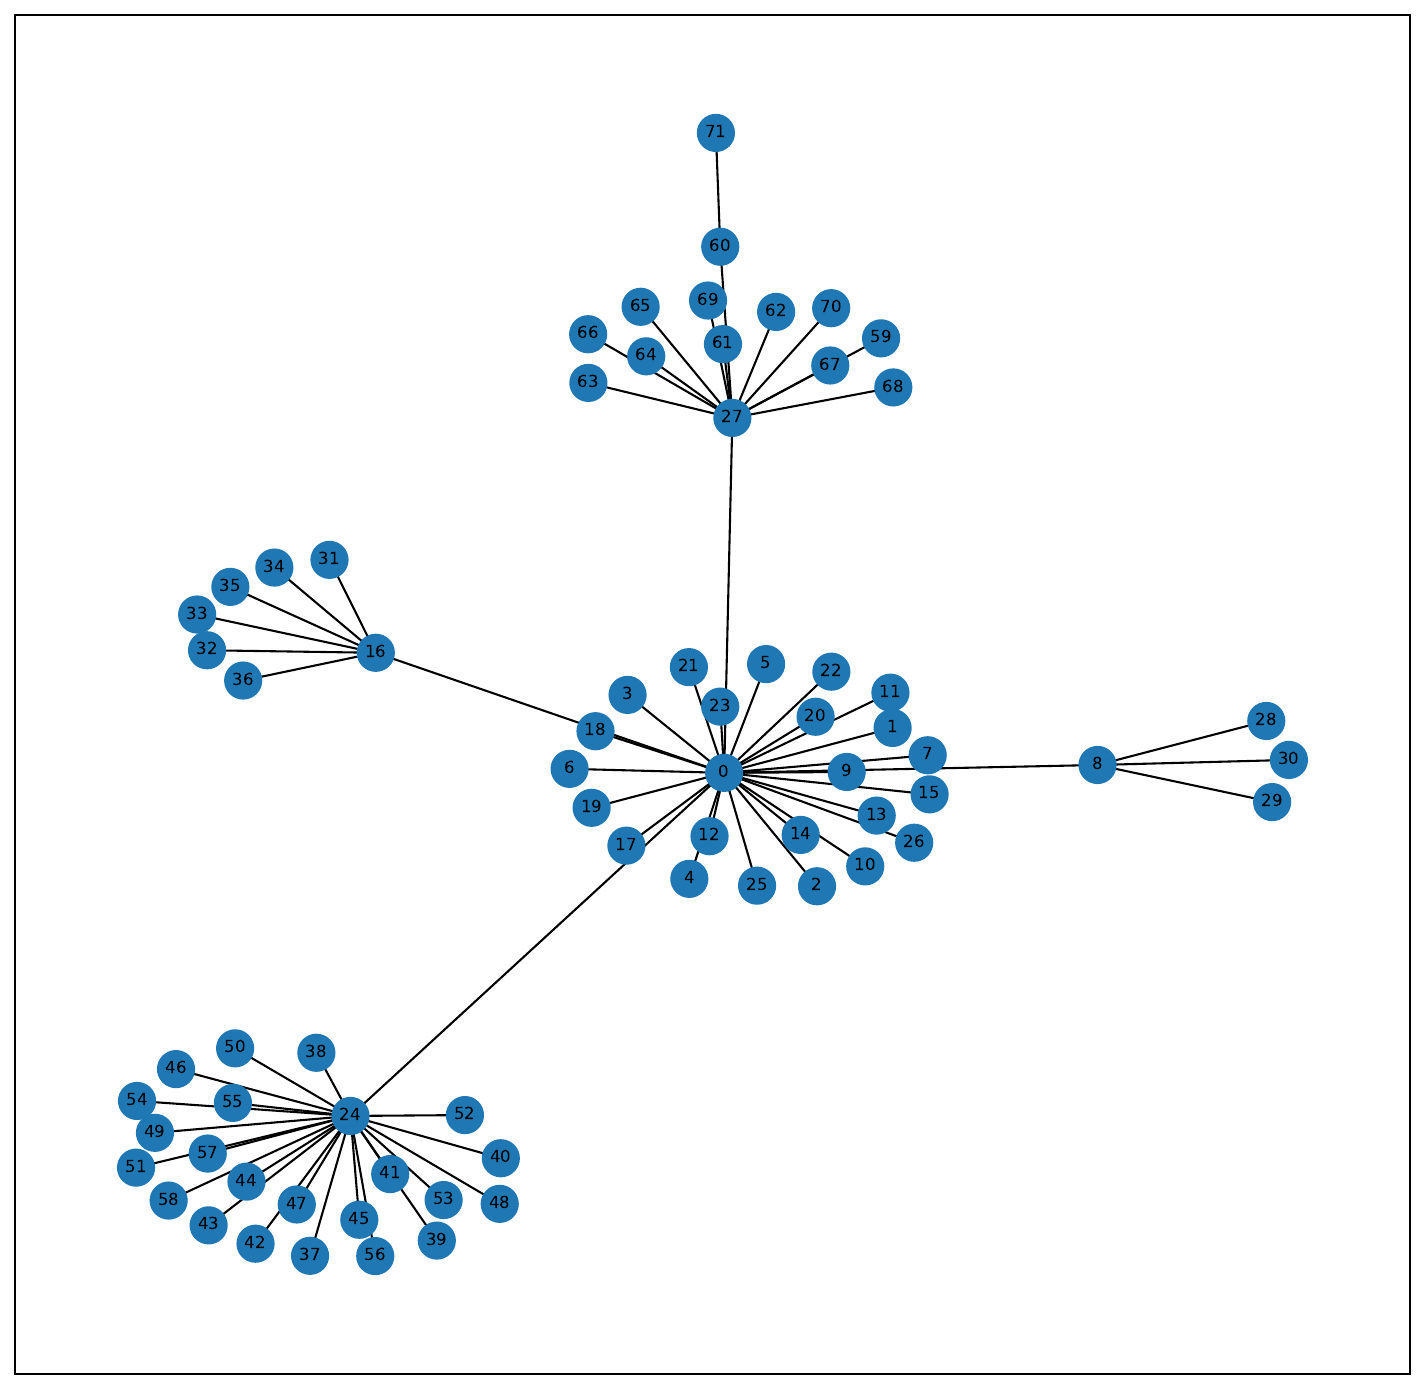
\includegraphics[scale=0.5]{EchoChamberExample1}
    \caption[Echo chamber example from UPFD-Politifact.]{A randomly sampled fake news instance that exhibits echo chamber behavior. Random sampling is made from UPFD-Politifact fake news instances. $0$-th node represents the root node with news embeddings. We will refer to this fake news example as the \emph{echo chamber example}.}
    \label{fig:echoChamberExample1}
\end{figure}
In the echo chamber example in~\ref{fig:echoChamberExample1}, it is trivial to observe some echo chambers created by nodes $24$, $27$, $16$, $8$ from biggest to smallest respectively. Furthermore, the initial spreaders of this example are assumed to be followers of the publisher of root node. Similar to this, there exist many features for this dataset.
Now that we have eloborated on the characteristics of our dataset, let us analyze whether these features were captured by our model. First, let us observe the explaining subgraph $\mathcal{G}_S$ in Fig~\ref{fig:EchoChamberExample1Explanation_no_threshold} for the echo chamber example.
\begin{figure}
    \centering
    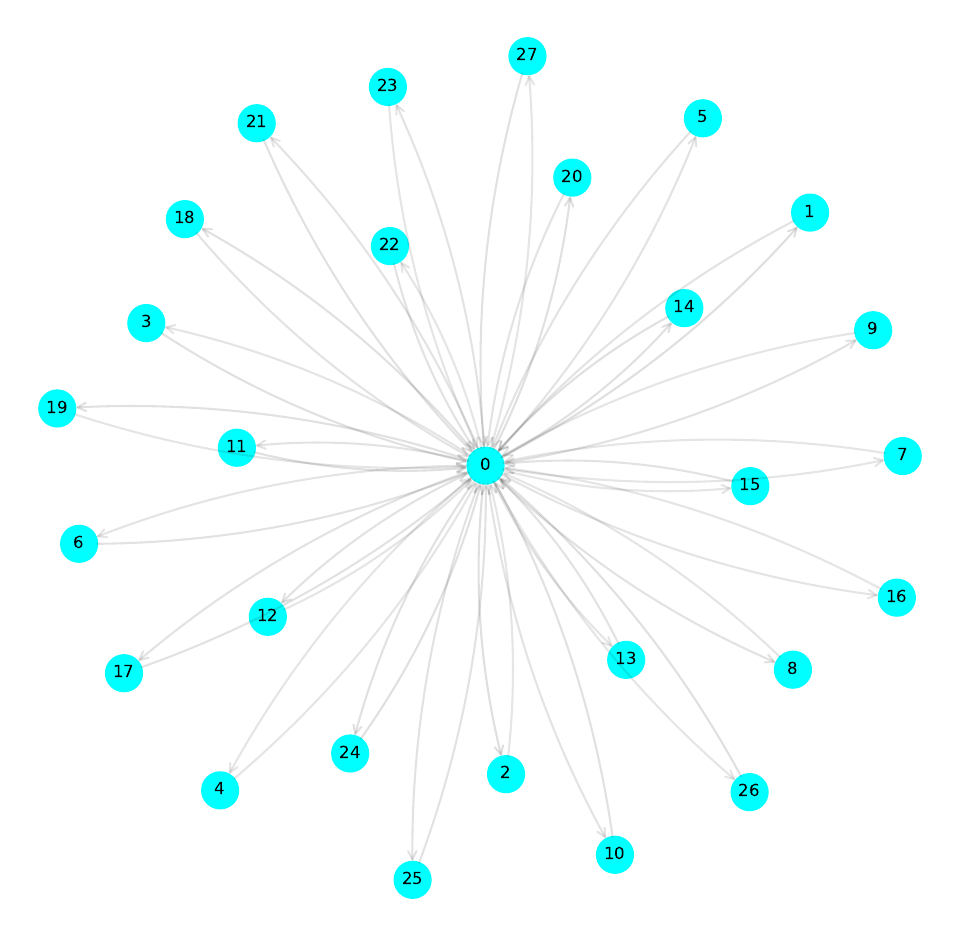
\includegraphics[scale=0.5]{EchoChamberExample1Explanation_no_threshold.png}
    \caption[Echo chamber example explanation for root node]{The explanation provided for our model and the echo chamber example for its root node. This instance was predicted as fake news with a probability of $0.9912$. Contains 27 nodes.}
    \label{fig:EchoChamberExample1Explanation_no_threshold}
\end{figure}
We first introduce how to interpret the explanation provided by GNNExplainer. Even though our dataset has undirected edges, we have obtained an explanation with bidirectional directed edges. To recap, undirected edges are interpreted as bidirectional edges, this is why GNNExplainer provided us with two edges per node pair. Additionally, there exist self-loops that simply is an edge from and to the same node $(v_i, v_i)$. The edge mask values for edges indicate the importance of the messages passed between two nodes. In order to understand the behavior of model in terms of the root node, we look at incoming edges to the root node in the explanation. Furthermore, the transparency of edges are an indicator for the magnitude of the edge mask value. However, this can not be clearly observed in this example.\\
On the other hand, when we look at the node feature mask $F$, we can understand which features are deemed important by our model for a given node. We are particularly interested in the root node, and the explanation associated to it. Since the root node consists of news content embeddings, intuitively, we can consider the root node explanation as the important subset of news content embeddings. However, we were not able to test this intuition due to (i) the size of data needed to be downloaded to construct FakeNewsNet~\parencite{FakeNewsNet_Shu} whose news content and social context data was utilized in our dataset, (ii) insufficient information on~\cite{UPFD_Dataset_Shu} to reproduce the UPFD framework, (iii) large maximum input sequence (768) for BERT model to process the news content on a local computer. Thus, we continue our analysis without considering node feature mask from now on. \\
\textbf{Interpreting the Explanation.} As one would expect, the model thinks that the the cascaders (initial retweeters) are the most important users (nodes) for the prediction of fake for this instance. Although there should be a significant difference in the edge mask values, specifically, since the spreaders are the users $v_8$, $v_{16}$, $v_{24}$, and $v_{27}$ we would expect larger importance scores on edges that connect these nodes to the root node. Interestingly, the edge $(v_0, v_{13})$ was assigned the highest edge mask value with $0.1371$. The edges $(v_0, v_8)$, $(v_0, v_{16})$, $(v_0, v_{24})$, and $(v_0, v_{27})$ were assigned $0.1081$, $0.0951$, $0.1222$, and $0.1181$, respectively.  While the reasons behind the maximal importance score assignment to edge $(v_0, v_{13})$ remains unclear, we observe that the biggest echo chamber's connection to the root node has a high edge mask value, which suggests that the model might be able to utilize the echo chambers with success for prediction. However, we need to observe similar behavior in other fake news instances that house echo chambers.\\
We also examined the highest edge mask valued five edges to understand which edges are important for our model. Before we proceed, it should be noted that the subgraph generation does not take into account where the maximal edge mask values reside, instead it tries to capture the biggest subgraph with the highest mutual information between the original graph and the subgraph with respect to the prediction.\\
\textbf{Edge Mask Analysis.} Proceeding our analysis for the five largest values in our edge mask provided by GNNExplainer, we observed that the second highest value belongs to the edge $(v_{24}, v_{41})$, i.e., an echo chamber connection. The third one belongs to a self-loop $(v_{44}, v_{44})$ and the fourth one is for the edge $(v_{44}, v_{24})$. We can interpret the edge mask value for the self-loop as the significance that model puts on the node $44$ ($v_{44}$). The edge mask value for edge $(v_{44}, v_{24})$ confirms our interpretation for node $v_{44}$, because this is the first instance for an important edge that is directed from a retweeter to its source. Thus, the user $v_{44}$ and their historical data should be investigated. The fifth largest edge mask value is assigned to the edge $(v_{27}, v_{62})$ which is another propagation edge in an echo chamber. The distribution of the edge mask values are given in Fig.~\ref{fig:EchoChamber1SubgraphEdgeMaskDistribution}\\
% \begin{figure}
%     \centering
%     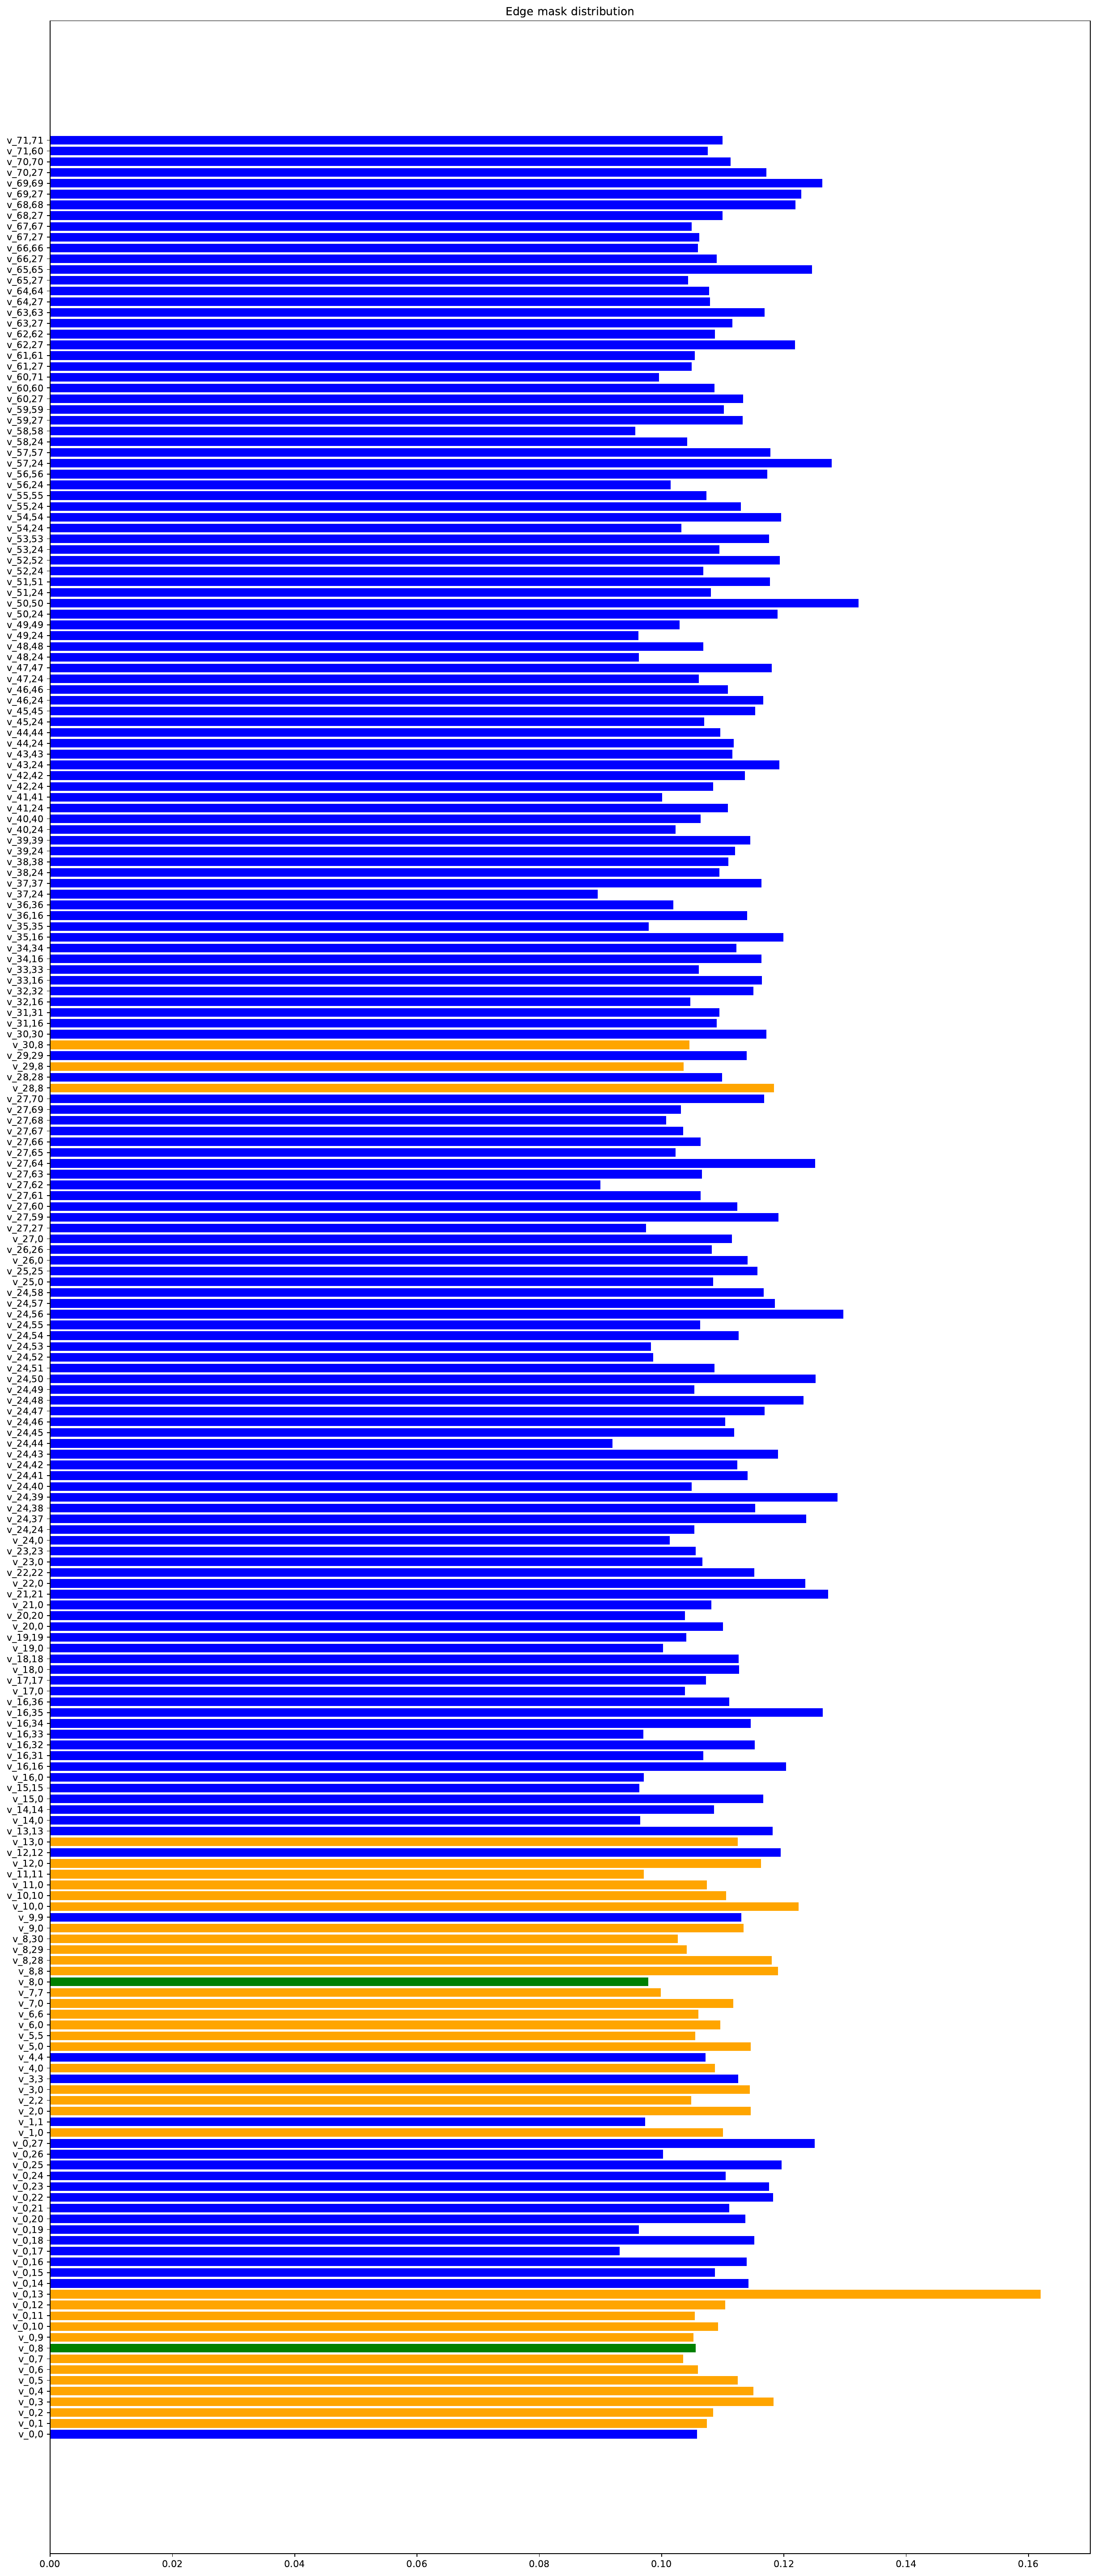
\includegraphics[scale=0.15]{EchoChamber1EdgeMaskDistribution.png}
%     \caption[Edge mask distribution of the input graph provided for echo chamber example explanation.]{Edge mask distribution of the input graph provided for echo chamber example explanation. The orange bars represent the edge mask values of the edges included in the subgraph explanation. Green bars indicate edges with the same characteristic as orange bars, but these edges are also connections to echo chambers.}
%     \label{fig:EchoChamber1EdgeMaskDistribution}
% \end{figure}
\begin{figure}
    \centering
    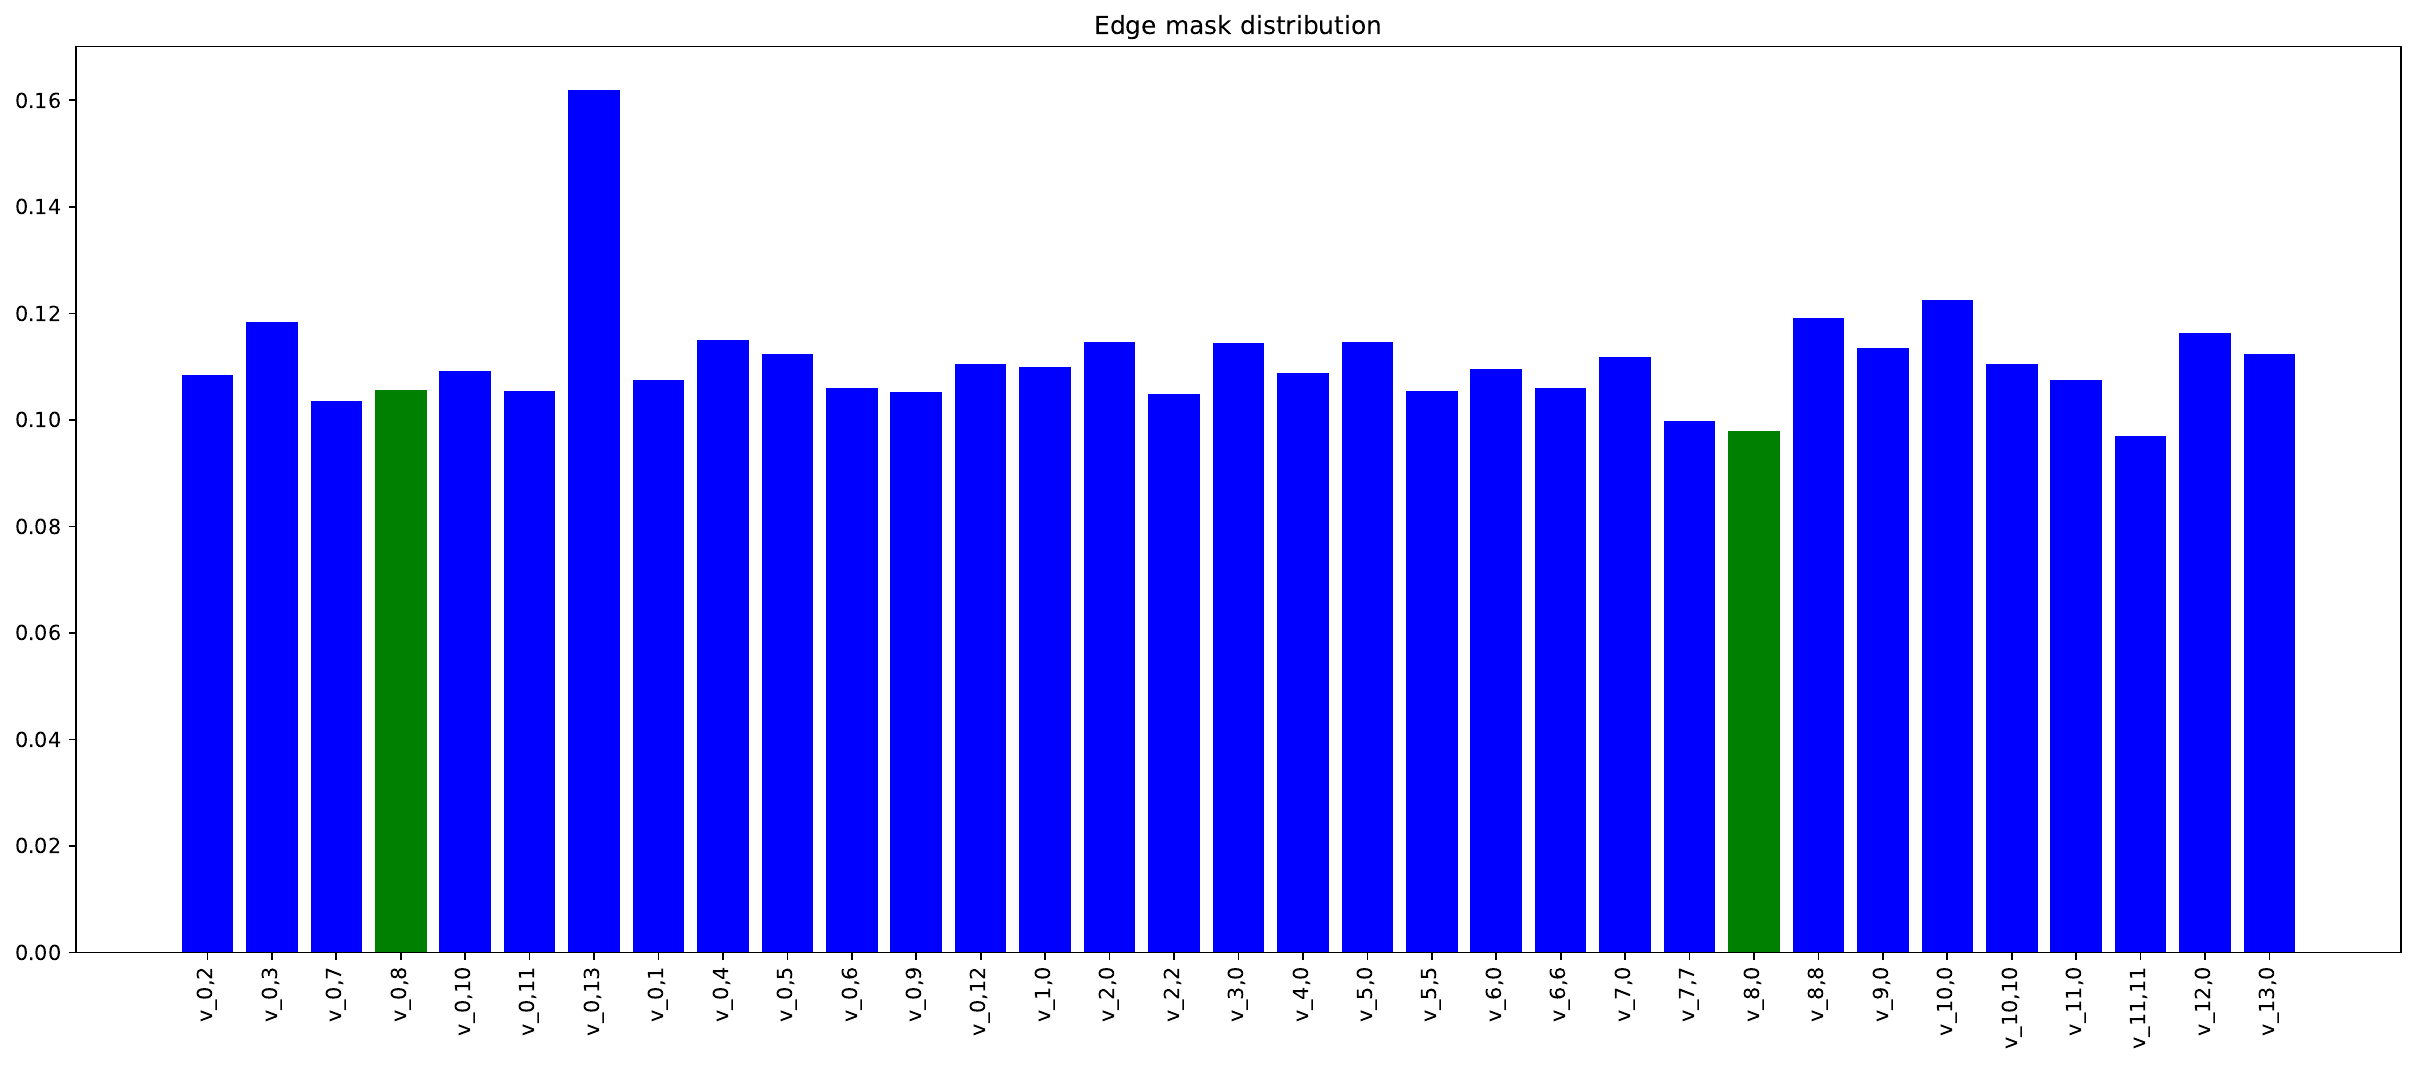
\includegraphics[scale=0.35]{EchoChamber1SubgraphEdgeMaskDistribution}
    \caption[Edge mask distribution of the subgraph provided for echo chamber example explanation.]{Edge mask distribution of the subgraph provided for echo chamber example explanation. The green bars represent the edge mask values of echo chamber connections.}
    \label{fig:EchoChamber1SubgraphEdgeMaskDistribution}
\end{figure}
Visiting back the features we introduced, we observe that the feature $SF_7$ is captured in this explanation. To elaborate, we see that the edges to the cascade node with the highest number of retweets were deemed important by the explainer. This implies that our model is able to capture important features. Although, in order to get this interpretation, one would require a data scientist. A domain expert or an end-user is likely to either misinterpret or not understand the explanation provided by GNNExplainer. Furthermore, some of the most important edges were not even included in the visualization. This certainly decreases the understandability of the explanations. \\
\textbf{Sensitivity Analysis.} We also analyzed the faithfulness of the explanations to the model. We took the explanation subgraph we provided in~\ref{fig:EchoChamberExample1Explanation_no_threshold}, restored its node features and fed it to model to see if the learned structure is still predicted as fake with high probability. In fact, the model predicted the subgraph as fake with $0.9915$ which is higher than the prediction probability of our instance. Overall, we say that the model is faithful to this instance,and GNNExplainer can indeed reduce noise in a graph as the authors claimed in~\cite{GNNExplainer_Ying}.\\
We proceed our analysis of this instance an experiment in which we remove the news content and historical information of children nodes both in the input and the explanation to see their effect on the prediction. We provide the results in Table~\ref{tab:echoChamberFeatureRemovalExperimentResults}.\\
\begin{table}
    \centering
    \begin{tabular}{c | c | c}
        \textbf{Operation}            & $p_{original}$ & $p_{subgraph}$ \\
        \hline
        No change                     & 0.9912         & 0.9915         \\
        \hline
        Remove news content           & 0.8328         & 0.8018         \\
        \hline
        Remove historical information & 0.9812         & 0.9809         \\
        \hline
        Remove all node information   & 0.4940         & 0.4940         \\
    \end{tabular}
    \caption[Model prediction probabilities for input perturbation experiment.]{Model prediction probabilities for input perturbation experiment. $p_{original}$ denotes prediction probability for the original input. Analogously, $p_{subgraph}$ refers to the prediction probability for the explanation subgraph.}
    \label{tab:echoChamberFeatureRemovalExperimentResults}
\end{table}
It is trivial to observe in Table~\ref{tab:echoChamberFeatureRemovalExperimentResults} that the model's confidence decreases as we remove news content for the echo chamber example. Interestingly, when we remove user historical information from all nodes except root node (root node contains the news content), the prediction probability does not drop too much. This suggests model takes into account the news content and structural information more than the historical information. This can also be observed from the model's architecture in Fig.~\ref{fig:UPFDClassifierArchitecture}. The skip connection and concatenation of the news content in the root node appears to be doing what is expected of it. In fact, the authors of UPFD~\parencite{UPFD_Dataset_Shu} showed that news content shows that with a vanilla version of UPFD classifier, i.e., without skip connection and concatenation, the performance drops. This finding of ours also goes in parallel with their finding. Furhtermore, when we remove all node information, the model loses can no longer tell fake from real. Thus, without node information, just depending on the structure and diffusion of a news piece for prediction turns out to be a bad idea. We certainly need some node embeddings, at least the embeddings for the news.\\
We illustrate more examples in order to understand if the statistically significant features were captured. First, it is nontrivial to look for $SF_1$ in the explanations as the tree depth will be decreased significantly. Most of the time the tree depth in the explanations we observed were 1. Thus, we skip this feature analysis. We look for the effect of feature $SF_2$ in the explanations. We make a simple comparison with our echo chamber example in Fig.~\ref{fig:echoChamberExample1} with a real news example in Fig.~\ref{fig:POL_RealNewsExample1}. The echo chamber example has 72 nodes whereas the real news example has 59 nodes. Now let us observe the explanation provided for the real news instance in Fig.~\ref{fig:POL_RealNewsExample1Explanation_no_threshold}.\\
\begin{figure}
    \centering
    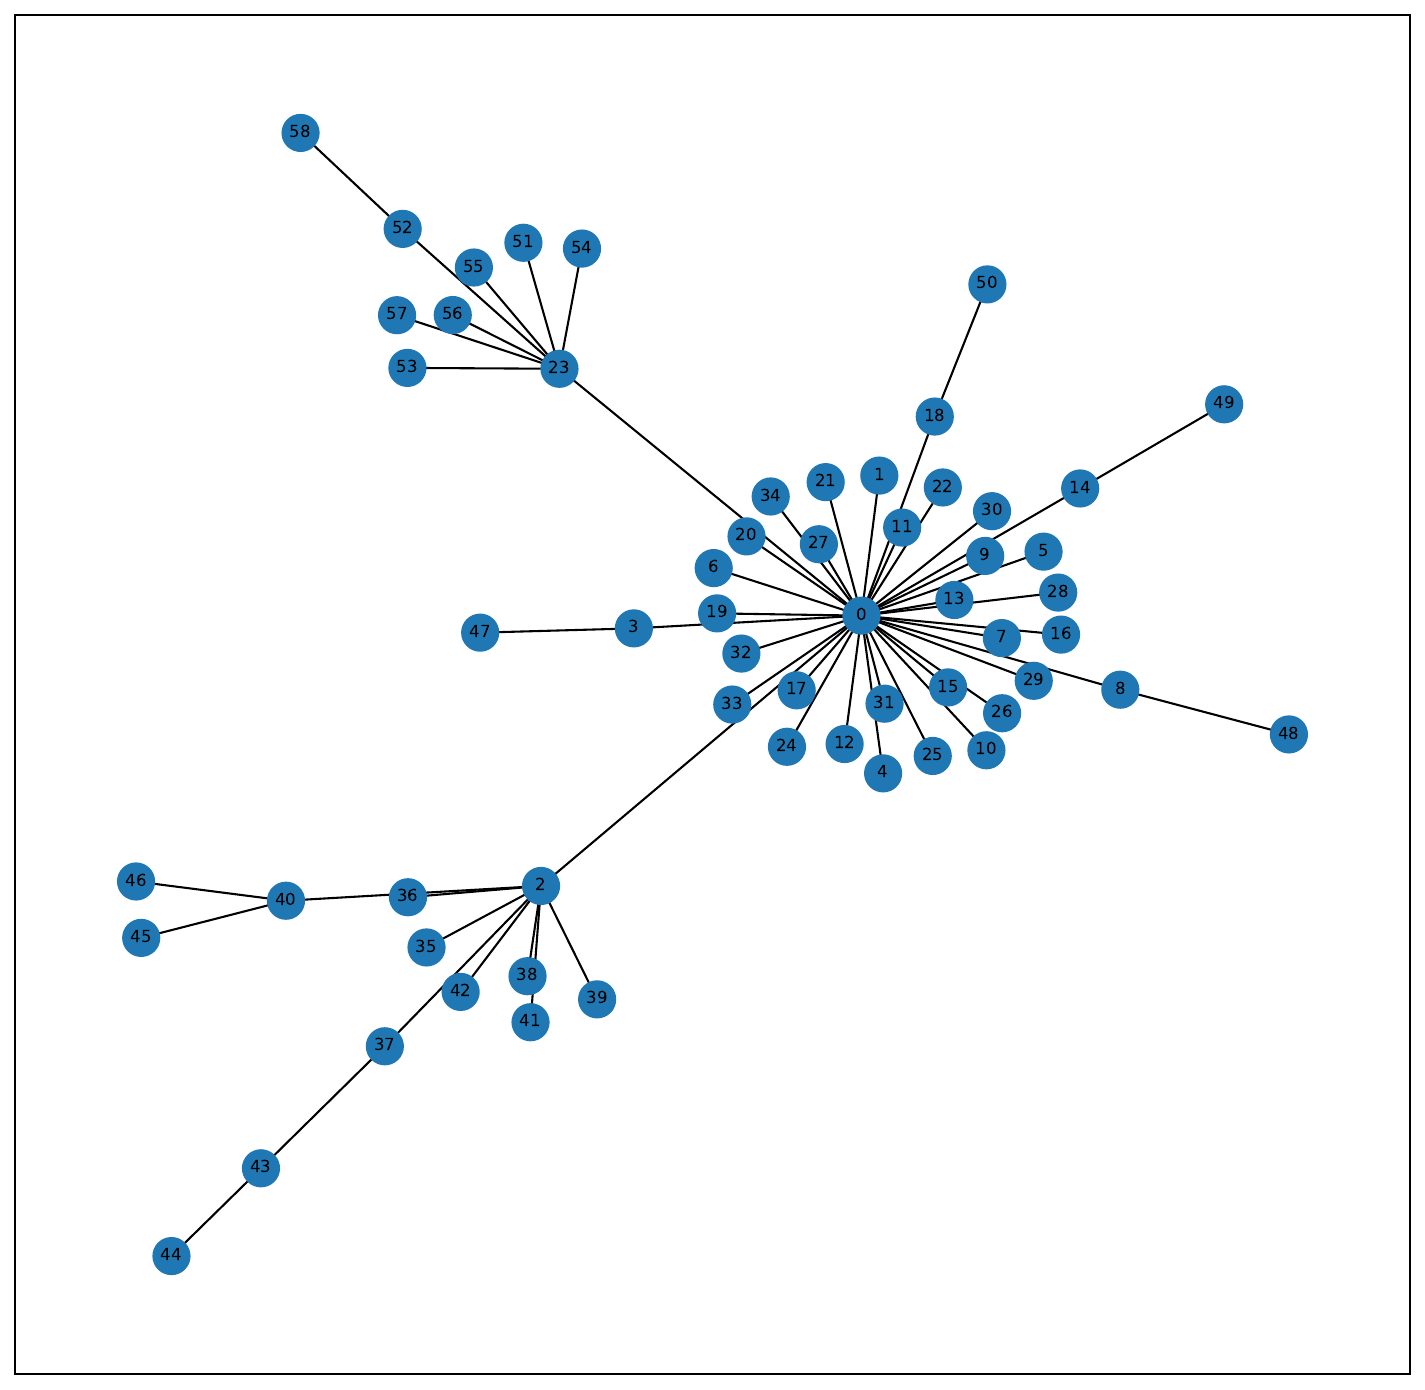
\includegraphics[scale=0.5]{POL_RealNewsExample1}
    \caption[A real news instance from UPFD-Politifact]{A real news instance from UPFD-Politifact. We shall refer to this example as the \emph{real news example}. It was predicted as real news with probability 0.9956}
    \label{fig:POL_RealNewsExample1}
\end{figure}
\begin{figure}
    \centering
    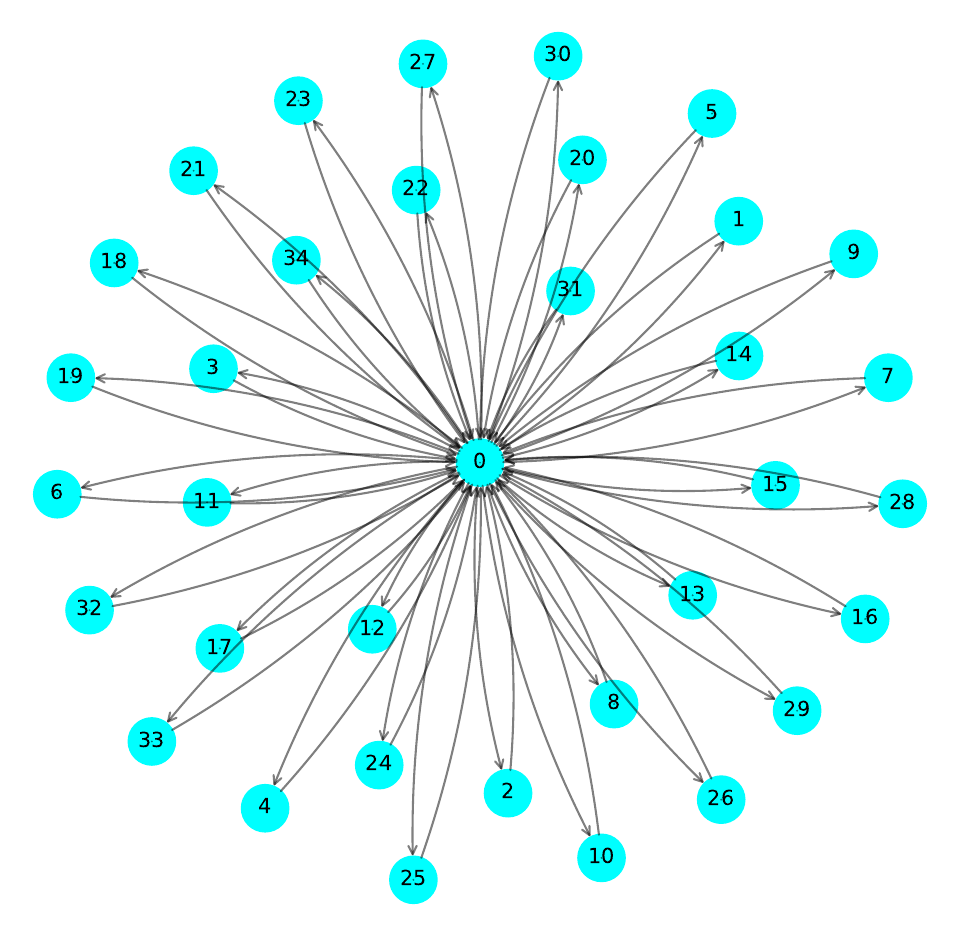
\includegraphics[scale=0.5]{POL_RealNewsExample1Explanation_no_threshold}
    \caption[Explanation for the real news example from UPFD-Politifact]{Explanation for the real news example from UPFD-Politifact. Contains 35 nodes.}
    \label{fig:POL_RealNewsExample1Explanation_no_threshold}
\end{figure}
The explanation subgraph for the real news example contains more nodes than the explanation subgraph for the echo chamber example. This might imply the effect of $SF_2$ on the explanations. In other words, explanations capture the importance of more nodes for the real news example. Although, this should be tested with other real and fake news instances to be verified. Furthermore, Although this instance has some nodes that create an echo chamber like effect, we can easily observe that some of these nodes were also retweeted, a behavior not observed in echo chamber example.\\
During our experiments, we realized that some explanations are hard to read, particularly the ones with too many nodes. Including the explanation provided in Fig.~\ref{fig:POL_RealNewsExample1Explanation_no_threshold}, it is hard to distinguish edges and nodes. In order to understand the importance of edges and simplify the explanation subgraph we employed three simple techniques in which we used a threshold value. Then we apply this threshold to the edge mask in which the values less than or equal to the threshold are set to zero. The first approach was straightforward, take the maximum value and set the threshold to a value less than that, and observe the changes in the explanation subgraph as we change the threshold value. The second approach is to get the mean of all edge mask values to get a threshold value. This way we obtain less edges in our initial explanation, but keeping an important set of edges to understand their importance. Our third approach is to take the median of the edge mask set, and use it as a threshold that applies the same effect as the averaging approach. There were no big differences between mean and median method. However, we opted for median as it was able to capture more edges for small explanation subgraphs. We illustrate the explanations with threshold methods mean and median in Fig~\ref{fig:POL_RealNewsExample1Explanation_with_threshold}.\\
\begin{figure}
    \centering
    \subfloat[Median]{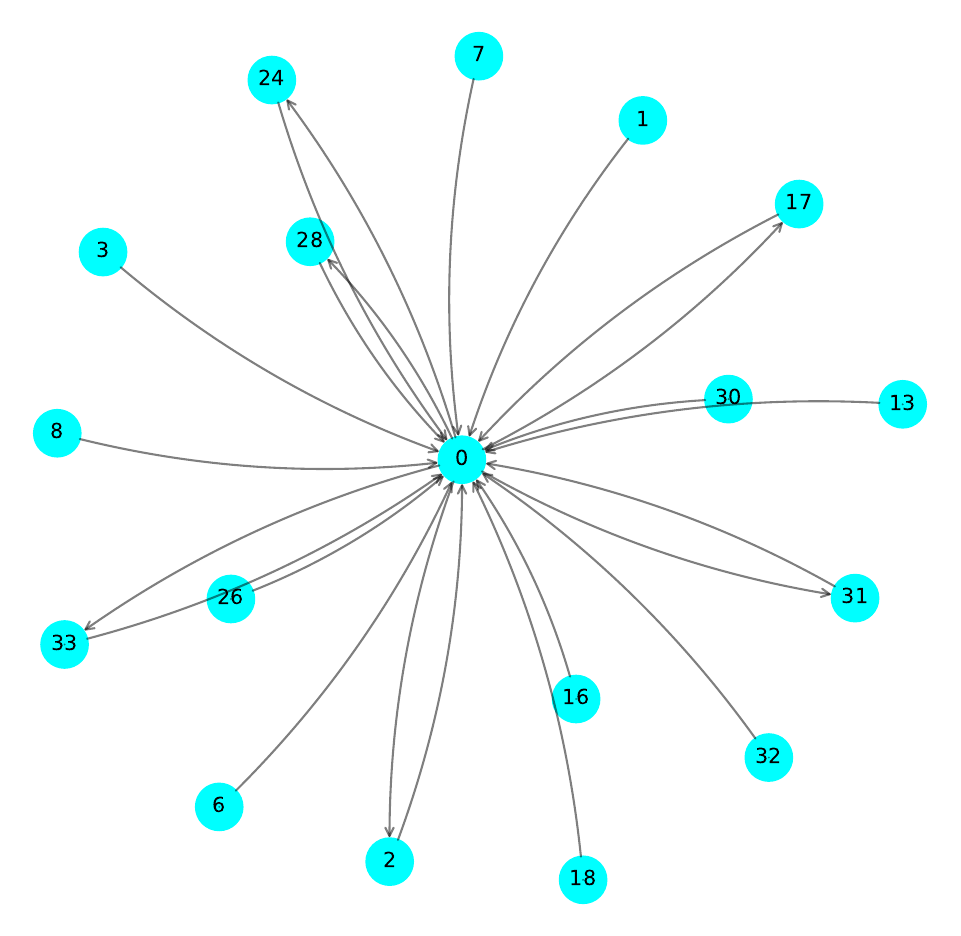
\includegraphics[width=0.45\textwidth]{POL_RealNewsExample1Explanation_with_threshold_median.png}}
    \hfill
    \subfloat[Mean]{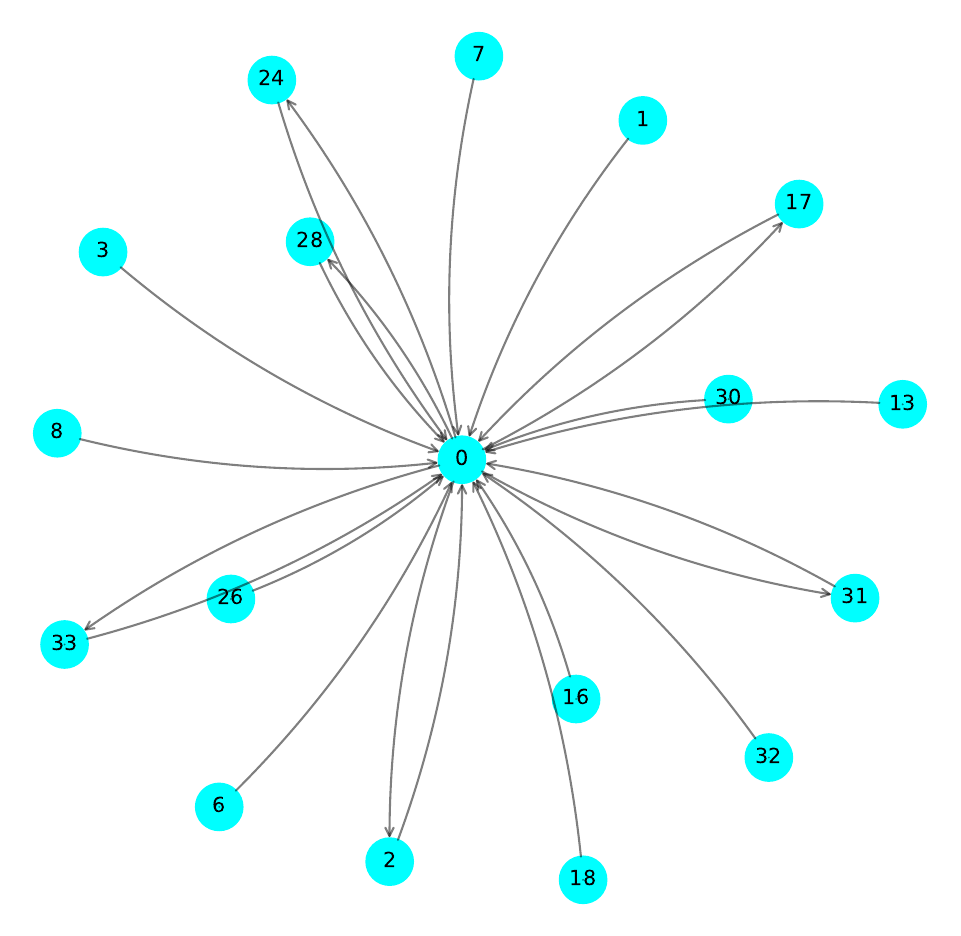
\includegraphics[width=0.45\textwidth]{POL_RealNewsExample1Explanation_with_threshold_mean.png}}
    \caption[Threshold methods for subgraph explanations of the real news example.]{Threshold methods for subgraph explanations of the real news example. In this case median and mean provides the same output.}
    \label{fig:POL_RealNewsExample1Explanation_with_threshold}
\end{figure}
We can extend our method to an interactive plot in which we are able to change the threshold value dynamically. Furhtermore, we can use the edge mask values provided for the edges in the subgraph to apply average and mean thresholding methods. We leave this for future work. \\
\textbf{Introducing Unseen Data.} We analyzed the predictions made for one real and one fake news instances that were in the test split. This time, we randomly sampled one fake news from the fake news set and one real news from the real news set in the test split of our UPFD-Gossipcop dataset which is unseen data for our model which was trained on the UPFD-Politifact dataset. We did not generate a new graph instance as obtaining the news piece, creating embeddings for it, and collecting its social context information is a very long process without some of this data prepared beforehand.\\
\begin{figure}
    \centering
    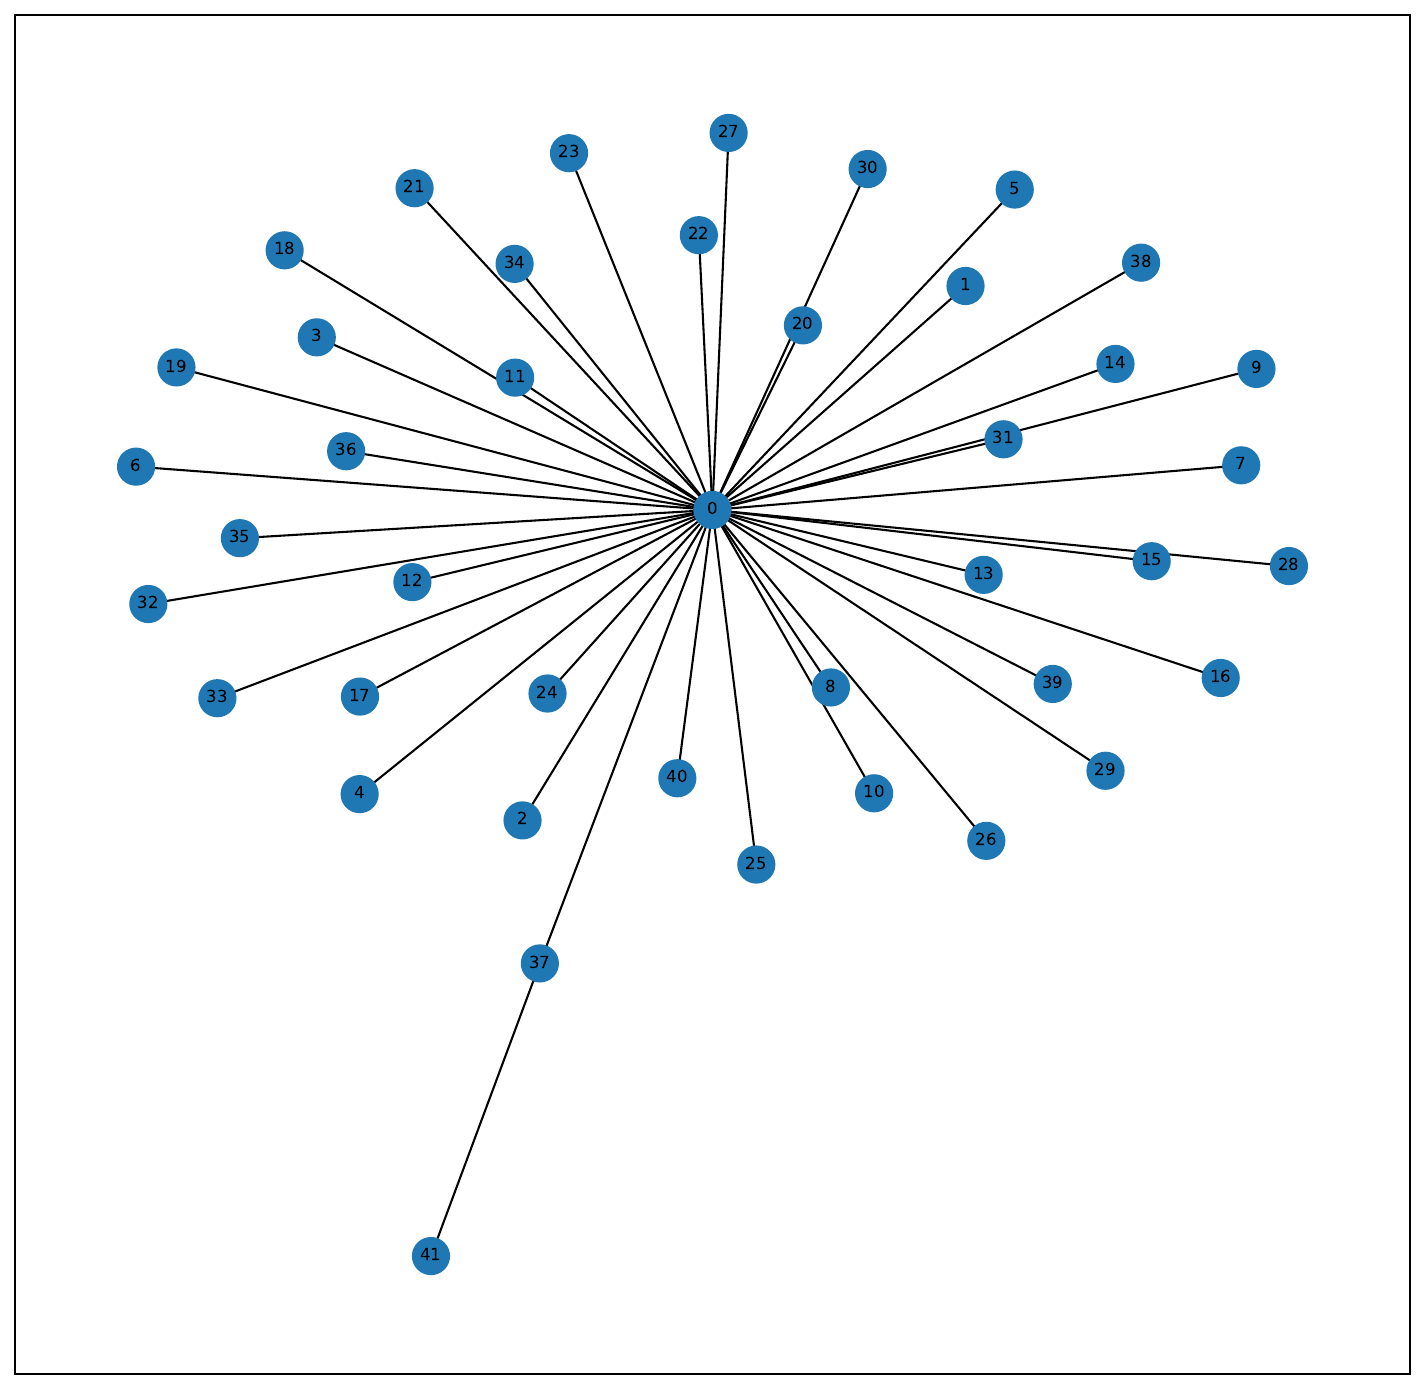
\includegraphics[scale=0.5]{GOS_FakeNewsExample1}
    \caption[A fake news example from UPFD-Gossipcop.]{A fake news example from UPFD-Gossipcop. We introduced this instance as an unseen data to our model, and it predicted this fake news piece as real with a probability of 0.9984.}
    \label{fig:GOS_FakeNewsExample1}
\end{figure}
Our fake news example from Gossipcop is illustrated in Fig.~\ref{fig:GOS_FakeNewsExample1}. It is obvious that this fake news piece does not display echo chamber patterns, in fact, structurally it looks more like a real news piece. This may be why our model mispredicted this instance. Let us further dive in to understand this. There can be a variety of reasons. It can be because of the difference in the news style in both datasets. Politifact houses a set of political news whereas Gossipcop houses a massive set of celebrity news. So the difference of textual structure could be a reason. Another reason can be the small number of training instances for the set. However, we were not able to gather suggestive information from the explanation thus we did not include the explanation. One way to understand whether the model responds to echo-chamber like structures is to create these echo chambers by adding children nodes to some of cascade nodes (initial retweeters) and feed this to the model. Thus, initially, we added 20 nodes with no information in them, and selected nodes $v_{37}$ and $v_{39}$ arbitrarily. The resulting graph is illustrated in Fig.~\ref{fig:GOS_FakeNewsExample1Perturbed}.
\begin{figure}
    \centering
    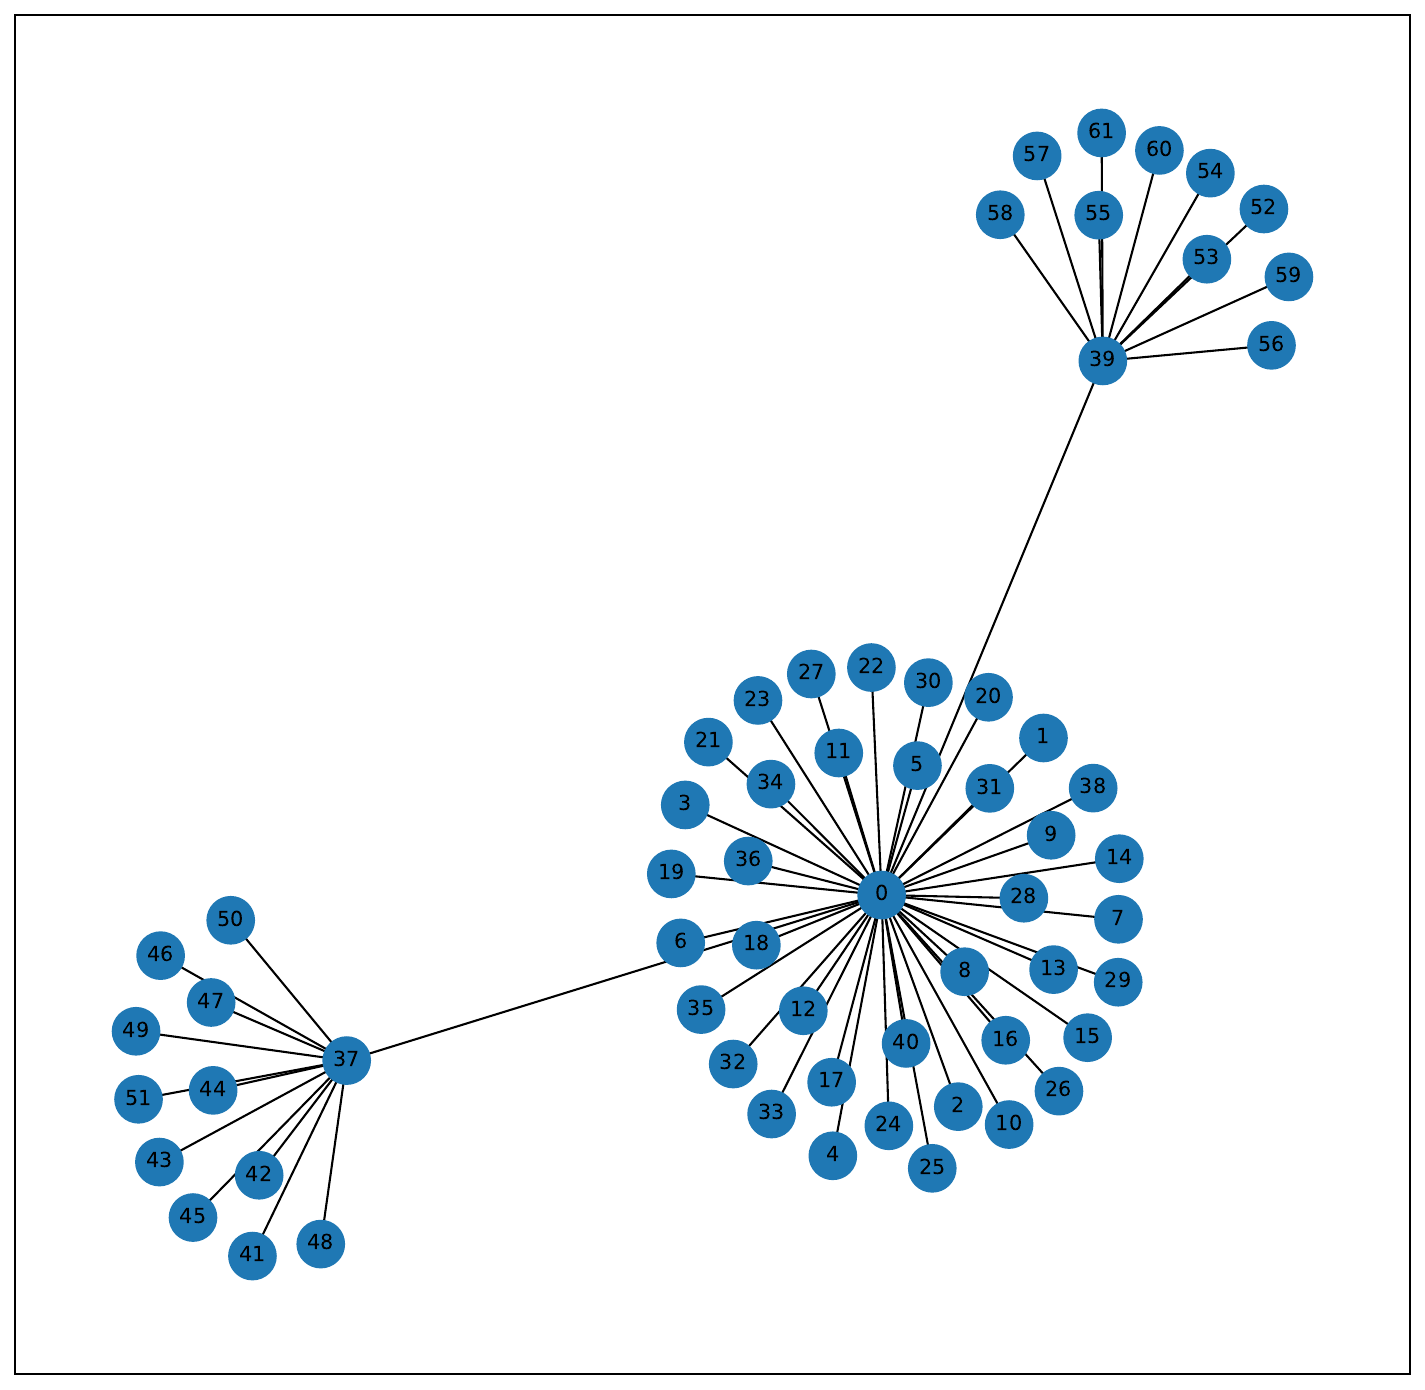
\includegraphics[scale=0.5]{GOS_FakeNewsExample1Perturbed}
    \caption[The perturbed version of the fake news example from UPFD-Gossipcop]{The perturbed version of the fake news example from UPFD-Gossipcop. We added echo-chamber like structures to nodes $v_{37}$ and $v_{39}$.}
    \label{fig:GOS_FakeNewsExample1Perturbed}
\end{figure}
When the fed the perturbed sample to our model, the increase in prediction probability for fake news unnoticably increased. So we also sampled some historical information from a randomly obtained fake news instance that is different than the one we are analyzing. We embedded the new nodes with randomly obtained user historical information. Then we fed this instance to the model, but the change in probability was too small to omit. Thus, for this instance our experiment suggests that echo-chamber like structures does not necessarily increase the probability for fake news.\\
% maybe include real news example from Gossipcop here.
\textbf{Latent Space Analysis.} We apply t-SNE~\parencite{tSNE_vanDerMaaten} using default settings provided by scikit-learn~\parencite{ScikitLearn_Pedregosa} to see if GraphSAGE is able to distinguish fake and real news before its outputs are concatenated with news content in the root node and then fed to the FCN. The visualization for this procedure is provided in Fig~\ref{fig:TSNE_GraphSAGE}.
\begin{figure}
    \centering
    \subfloat[Gossipcop]{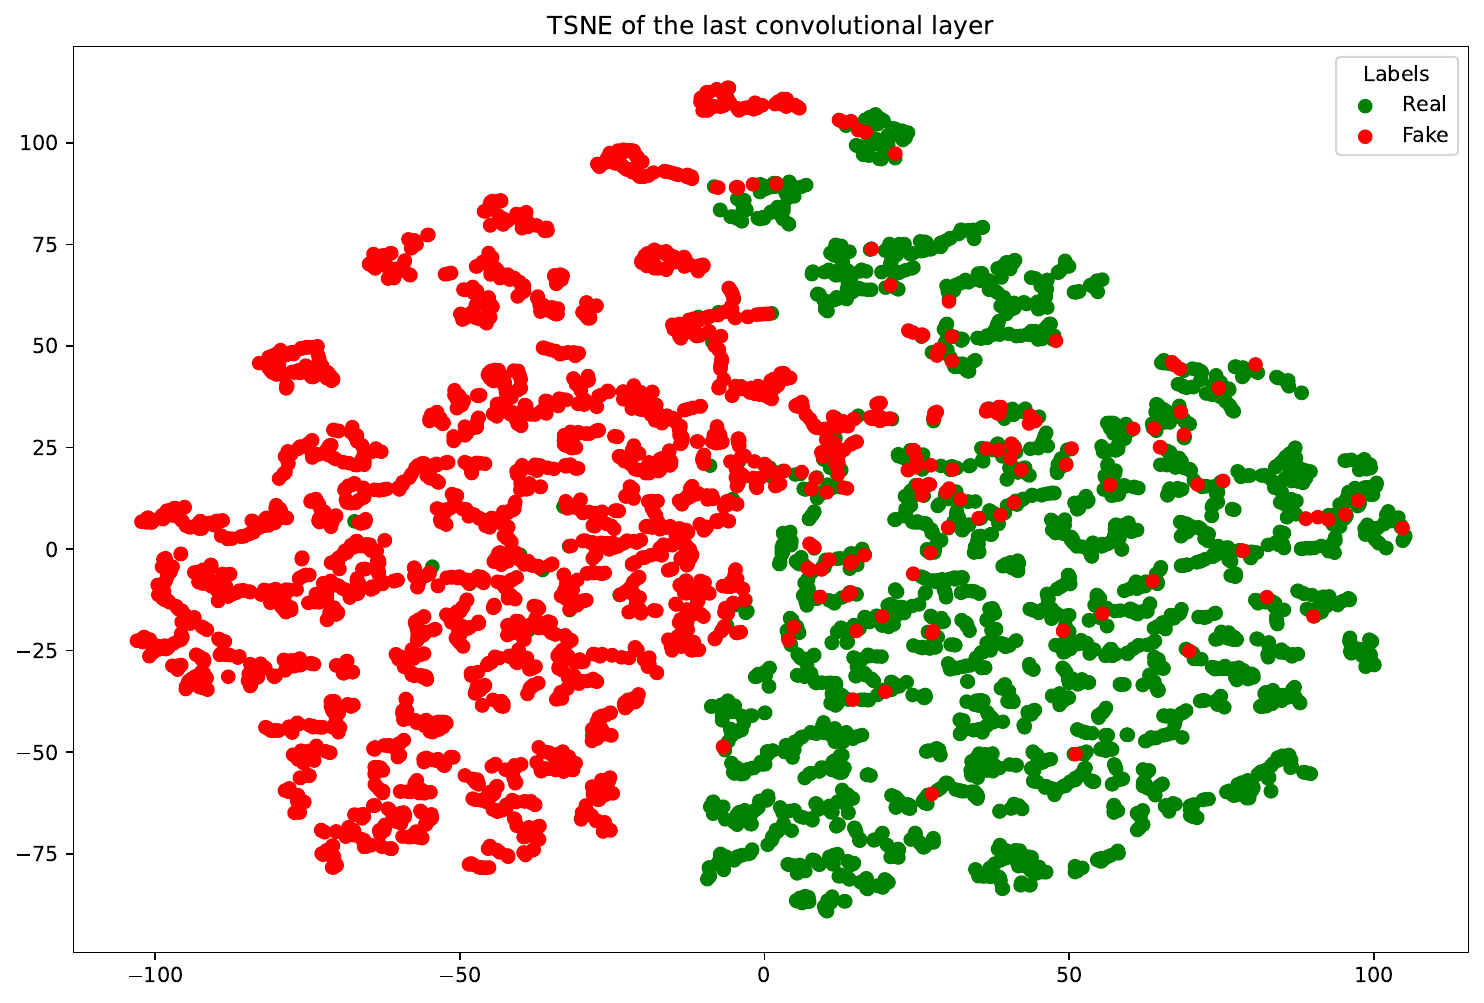
\includegraphics[width=0.45\textwidth]{TSNE_GraphSAGE_GOS.png}\label{subfig:TSNE_GraphSAGE_GOS}}
    \hfill
    \subfloat[Politifact]{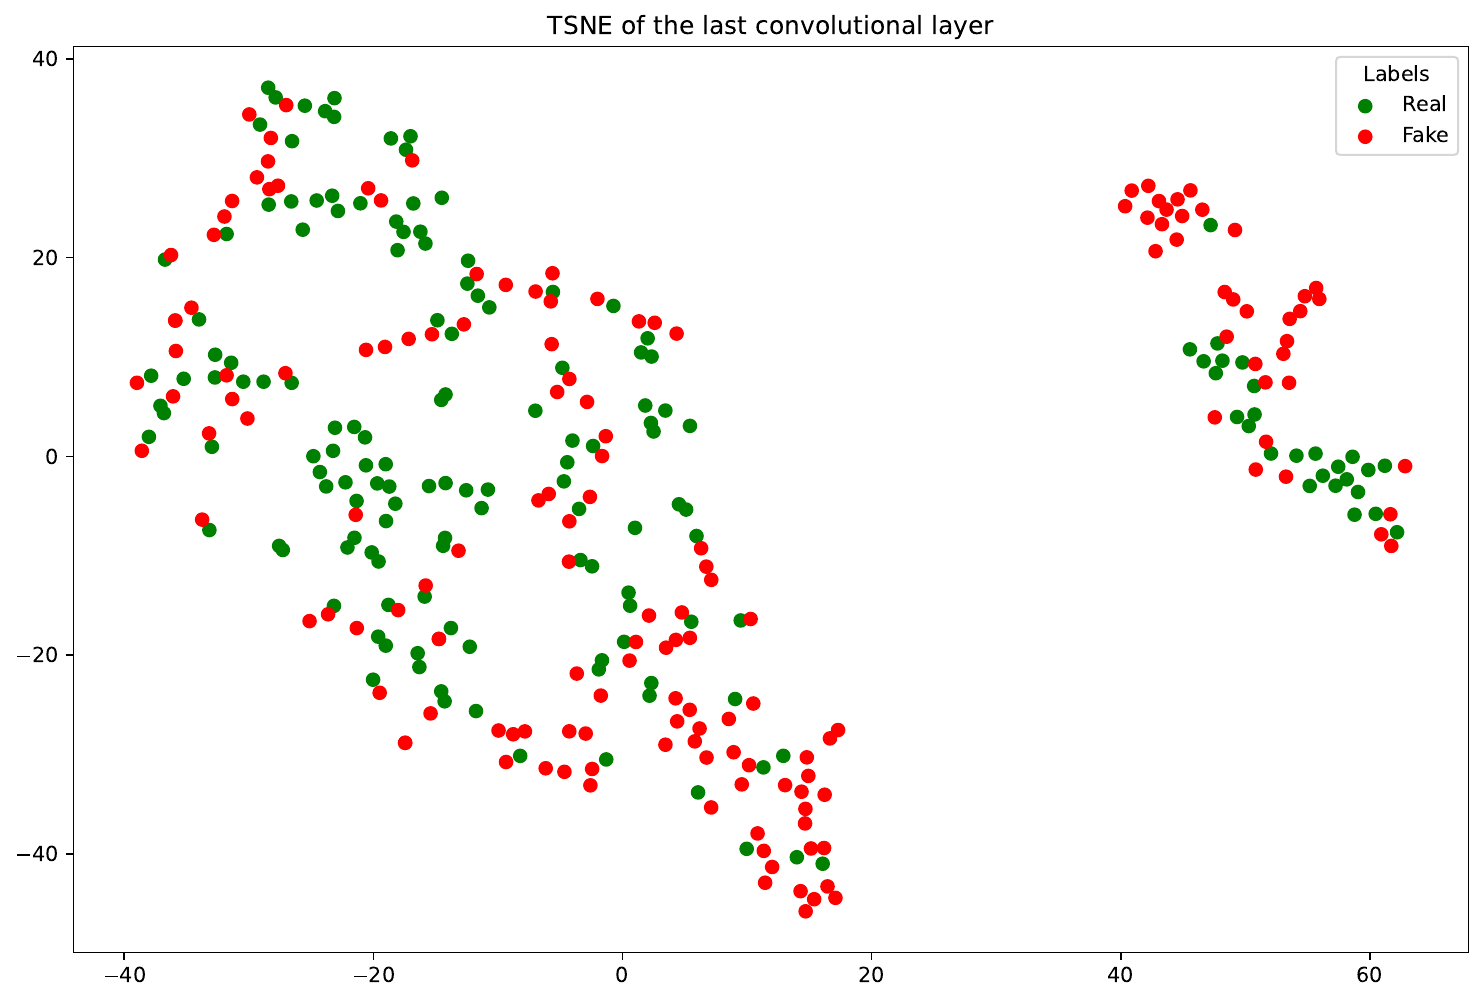
\includegraphics[width=0.45\textwidth]{TSNE_GraphSAGE_POL.png}\label{subfig:TSNE_GraphSAGE_POL}}
    \caption[t-SNE visualizations for GraphSAGE]{t-SNE visualizations for max pooled GraphSAGE on UPFD.}
    \label{fig:TSNE_GraphSAGE}
\end{figure}
Clearly GraphSAGE is able to distinguish fake and real news instances better in Gossipcop dataset, but it fails to make this discirimination with Politifact dataset. This can be due to the low amounts of instances in the Politifact dataset.\\
\textbf{Target Audience and XAI Goals for GNNExplainer.} It is quite clear that understanding the model's behavior locally with just a visualization is not sufficient for an end-user to understand why a particular news piece was predicted as real or fake. However, given enough resources, one can reverse engineer the process in the UPFD framework, which would allow for the analysis of node feature masks of news content and historical information embeddings. That would certainly increase the trustworthiness and informativeness of the model. We also suggest to employ interactive visualizations when working with GNNExplainer since the explanations can get very big. Explanations produced by GNNExplainer should be investigated by a data scientist who will simplify the explanation for a domain expert or an end-user. For our dataset, this simplification process can include aggregation of bidirectional edge mask values so that they can be represented as an undirected edge. Moreover, these undirected edges can be color-coded such that each color represents a value above a certain threshold which can be obtained using the methods we suggested. Also for GNNs with language models, the node feaures should be easily mappable to the textual content in such a way that we can create a variation of force plots provided by SHAP framework.\\
To sum up, we have analyzed the explanations produced by GNNExplainer for our model which was trained on UPFD-Politifact dataset. We have observed some of the statistically significant features' existence in the explanations. We have also addressed shortcomings of GNNExplainer, suggested simple yet effective methods to reduce the complexity of an explanation. All experiments were conducted using Python 3.7~\parencite{Python_Rossum}, PyTorch 1.11.0~\parencite{PyTorch_Paszke} and PyTorch Geometric 2.0.4~\parencite{PyTorchGeometric_Fey}. All visualizations were obtained through the use of NetworkX 2.6.3~\parencite{NetworkX_Hagberg} and Matplotlib 3.5.1~\parencite{Matplotlib_Hunter}. The detailed library usage and the implementation of all models are provided in our github repository~\footnote{\url{https://github.com/sersery35/Explainability_of_FND_Models/tree/main/GNNFakeNews}}.